% ---- ETD Document Class and Useful Packages ---- %
\documentclass{ucetd}
%\usepackage{oneinchmargins}
\usepackage{times}
\usepackage{relsize}
\usepackage{enumerate}
\usepackage{graphicx}
\usepackage{url}
%\usepackage{color}
\usepackage[usenames,dvipsnames]{xcolor}
%\usepackage[pagebackref]{hyperref}
%\usepackage[bookmarks=false]{hyperref}

%\hypersetup{colorlinks=true,citecolor=OliveGreen,linkcolor=Maroon,urlcolor=NavyBlue}

%\hypersetup{colorlinks=true,
%citecolor=Maroon,
%linkcolor=Green,
%urlcolor=Maroon}

%\usepackage{breakurl}
\usepackage{setspace}
\usepackage{rotating}

\usepackage{floatflt}
\usepackage{wrapfig}
\usepackage{alltt}
\usepackage{epstopdf}
\usepackage{subfigure}

%\usepackage{listings}
%\usepackage{algorithm}
%\usepackage{algorithmic}

\usepackage{fancyvrb}
%\usepackage{ulem} % for strike out,  
% \em and \sout are now strikes, use \it for italic
% never do this because now all 
\renewcommand{\ttdefault}{cmtt}

%\usepackage{colortbl} % for table color
%\usepackage{pstricks} % for gray hline
%\input{colortab} % for gray hline (must include pstricks)
%\usepackage{array}



% make sure url bib break point does not
% give undefull hbox message and the break line 
% is really nice now
\usepackage{etoolbox}
\apptocmd{\thebibliography}{\raggedright}{}{}


% -----------------------------------------------------
\usepackage{rotating}

\usepackage{subfigure,epsfig,amsfonts}
\usepackage{natbib}
\usepackage{amsmath}
\usepackage{amssymb}
\usepackage{amsthm}


% ---------------------------------------------
% name abbrvs .. 
% ---------------------------------------------
\newcommand{\infokernel}{\mbox{infokernel}}
\newcommand{\unix}{{\sc Unix}}
\newcommand{\dare}{DARE}
\def \samc {\textsc{SamC}}
\def \sampro {\textsc{SamPro}}
\def \samzoo {\textsc{SamZoo}}
\def \sammr {\textsc{SamMr}}
\def \sammace {\textsc{SamMace}}
\def \samcass {\textsc{SamCass}}
\def \sameiger {\textsc{SamEiger}}
\def \modist {\textsc{Modist}}
\def \macemc {\textsc{MaceMC}}
\def \setsudo {\textsc{Setsudo}}
\def \prefail {\textsc{PreFail}}

\def \fate {\textsc{Fate}}
\def \late {\textsc{Late}}
\def \lights {\textsc{LigHTS}}

\def \taxdc {TaxDC}
\def \tdc {TaxDC}
\def \sck {\textsc{SCk}}
\def \cdb {\textsc{CbsDB}}
\def \cbs {CBS}

\newcommand{\ts}[1]{{\tt{\small#1}}}


\def \uuu {\textbf{\textcolor{Maroon}{\textbf{$\uparrow$}}}}
\def \uu {\textbf{\textcolor{Maroon}{\textbf{$\Uparrow$}}}}
% \def \nu {\textbf{\textcolor{Maroon}{\textbf{$\nearrow$}}}} % submission only

\def \sleep {\ts{sleep()}}

\newcommand{\num}[1]{\textcolor{red}{\textbf{#1}}}
\def \numOldDeepBugs {12} 
\def \numZkDeepBugs {7}   
\def \numMrDeepBugs {3}
\def \numCsDeepBugs {2}
\def \numZkNewBugs {1}
\def \numMrNewBugs {1}
\def \numNewBugs {2}
\def \numVersions {10}
\def \numLinesSamPro {10,886}
\def \numProtocols {7}
\def \numLinesRule {35}  
\def \numMaxBugSpeedUp {271x}  
\def \numAvgBugSpeedUp {33x}    
\def \numAvgExecTime {40}

\def \numMinRedRatio {37x}  
\def \numMaxRedRatio {166x}  
\def \numRedRatioExecs {3000}

%\newcommand{\mrb}[1]{MR-#1}
%\newcommand{\zkb}[1]{ZK-#1}
%\newcommand{\zk}[1]{ZooKeeper-#1}
%\newcommand{\mr}[1]{MapReduce-#1}
%\newcommand{\cs}[1]{Cassandra-#1}

\newcommand{\jira}[3]{\href{http://issues.apache.org/jira/browse/#1-#3}{#2-#3}}

\newcommand{\mrb}[1]{\jira{MAPREDUCE}{MR}{#1}}
\newcommand{\zkb}[1]{\jira{ZOOKEEPER}{ZK}{#1}}
\newcommand{\cab}[1]{\jira{CASSANDRA}{CA}{#1}}
\newcommand{\hbb}[1]{\jira{HBASE}{HB}{#1}}
\newcommand{\hdb}[1]{\jira{HDFS}{HD}{#1}}
\newcommand{\zk}[1]{\jira{ZOOKEEPER}{ZK}{#1}}
\newcommand{\mr}[1]{\jira{MAPREDUCE}{MR}{#1}}
\newcommand{\ca}[1]{\jira{CASSANDRA}{CA}{#1}}
\newcommand{\hb}[1]{\jira{HBASE}{HB}{#1}}
\newcommand{\hd}[1]{\jira{HDFS}{HD}{#1}}


\def \ll {\ts{L}}
\def \ff {\ts{F}}
\def \pri {\ts{pr}$_{i}$}
\def \prone {\ts{pr}$_{1}$}
\def \prtwo {\ts{pr}$_{2}$}
\def \prtri {\ts{pr}$_{3}$}

\def \ls {\ts{ls}}
\def \als {\ts{als}}
\def \rals {\ts{rals}}
\def \ralsi {\ts{rals}$_{i}$}
\def \ralsone {\ts{rals}$_{1}$}
\def \ralstwo {\ts{rals}$_{2}$}
\def \ralstri {\ts{rals}$_{3}$}
\def \rags {\ts{rags}}


\def \gs {\ts{gs}}
\def \ags {\ts{ags}}
\def \nn {\ts{N}}
\def \none {\ts{N1}}
\def \ntwo {\ts{N2}}
\def \ntri {\ts{N3}}
\def \nfour {\ts{N4}}
\def \mone {\ts{m}$_{1}$}
\def \mn {\ts{m}$_{n}$}
\def \mm {\ts{m}}
\def \fone {\ts{F1}}
\def \ftwo {\ts{F2}}
\def \ftri {\ts{F3}}
\def \ma {\ts{a}}
\def \mb {\ts{b}}
\def \mc {\ts{c}}
\def \md {\ts{d}}
\def \mx {\ts{m1}}
\def \my {\ts{m2}}
\def \xx {\ts{X}}
\def \pg {\ts{pg}}
\def \pl {\ts{pl}}
\def \pp {\ts{p}}
\def \pd {\ts{pd}}
\def \pi {\ts{pi}}
\def \pm {\ts{pm}}
\def \pc {\ts{pc}}

% ---------------------------------------------
% spaces
% ---------------------------------------------
\newcommand{\vtwenty}{\vspace{20pt}}
\newcommand{\vfifteen}{\vspace{15pt}}
\newcommand{\vten}{\vspace{10pt}}
\newcommand{\vfive}{\vspace{5pt}}
\newcommand{\vthree}{\vspace{3pt}}

\newcommand{\vmintwo}{\vspace{-2pt}}
\newcommand{\vminthree}{\vspace{-3pt}}
\newcommand{\vminfive}{\vspace{-5pt}}
\newcommand{\vminten}{\vspace{-10pt}}
\newcommand{\vminfifteen}{\vspace{-15pt}}
\newcommand{\vmintwenty}{\vspace{-20pt}}

% ---------------------------------------------
% overloaded commands
% ---------------------------------------------
\newcommand{\ub}[1]{\underline{{\bf #1}}}
\newcommand{\bquote}{\vspace{-0.25cm} \begin{quote}}
\newcommand{\equote}{\end{quote}\vspace{-0.2cm} }
\def \sec {\S}
\def \yes {$\surd$}

\def \nospace {
  \setlength{\itemsep}{0pt}
  \setlength{\parskip}{0pt}
  \setlength{\parsep}{0pt}
}


\newcommand{\supsection}[1]{\noindent{\Large{\bf #1}}\vten}

\newenvironment{enumerate2}{
  \begin{enumerate}
  \setlength{\itemsep}{1pt}
  \setlength{\parskip}{0pt}
  \setlength{\parsep}{0pt}
}{
  \end{enumerate}
}

\newenvironment{itemize2}{
  \begin{itemize}
 \renewcommand{\labelitemi}{-}
  \setlength{\itemsep}{1pt}
  \setlength{\parskip}{0pt}
  \setlength{\parsep}{0pt}
}{
  \end{itemize}
}

% \renewcommand\thesection{\Alph{section}}



% ---------------------------------------------
% note
% ---------------------------------------------
\newcommand{\hsg}[1]{\textcolor{red}{{\small {\bf (HSG: #1)}}}}
\newcommand{\tl}[1]{\textcolor{red}{{\small {\bf (TL: #1)}}}}
\newcommand{\pj}[1]{\textcolor{red}{{\small {\bf (PJ: #1)}}}}
\newcommand{\thanh}[1]{\textcolor{red}{{\small {\bf (THANH: #1)}}}}
\newcommand{\todo}[1]{\textcolor{red}{{\small {\bf (TODO: #1)}}}}
%\newcommand{\newtext}[1]{\textcolor{blue}{#1}}
\newcommand{\newtext}[1]{#1}
\newcommand{\bluetext}[1]{\textcolor{blue}{#1}}
\newcommand{\rbt}[1]{\textcolor{red}{\textbf{#1}}}
\newcommand{\notes}[1]{\textcolor{darkgray}{
{\footnotesize {\em (Notes: #1)}}}}






% ---------------------------------------------
% bullets
% ---------------------------------------------
\def \vvvnb {\vfifteen \noindent $\bullet$~}
\def \vvnb {\vten \noindent $\bullet$~}
\def \vnb {\vfive \noindent $\bullet$~}

\def \tb {\vspace{8pt}\nb}

\def \vvn {\vten \noindent}
\def \vn {\vfive \noindent}
\def \nb {\noindent $\bullet$~}
\def \ni {\noindent}



% ---------------------------------------------
% counters, steps, hypothesis, tasks
% ---------------------------------------------
\newcommand{\hypo}[1]{
\begin{quote}
\stepcounter{HYPO}{\bf Hypothesis \arabic{HYPO}:} 
{\em #1}
\end{quote}
}

\newcommand{\taskformat}[2]{#1\textsc{#2}}

\newcommand{\task}[3]{
\begin{quote}
\phantomsection
\hypertarget{task#1#2}{}
{\bf Task \taskformat{#1}{#2}:} 
{\em #3}
\end{quote}
}

\newcommand{\tasklink}[2]{\hyperlink{task#1#2}{\taskformat{#1}{#2}}}

\newcounter{HYPO}
\newcounter{TASK}

\newcommand{\rs}{{ResearchStaff$_1$}}
\newcommand{\raOne}{{\bf RA$_1$}}
\newcommand{\raTwo}{{\bf RA$_2$}}
\newcommand{\ndv}{{\bf NDV}}
\newcommand{\ug}{{\bf Undergrad$_1$}}


% ---------------------------------------------
% extra sections, pages
% ---------------------------------------------

\newcommand{\sssubsection}[1]{\vten\textbf{\large{\textsc{#1}}}}


\newcommand{\emptypage}{
\newpage
\thispagestyle{empty}
(empty page)
}


% ---------------------------------------------
% figs
% ---------------------------------------------
\newcommand{\myrotate}[1]{\begin{rotate}{90} {\bf #1} \end{rotate}}

\newcommand{\mycaption}[4][]{%
\ifthenelse{\equal{#1}{}}{
\begin{spacing}{0.95}
\caption{
\label{#2}
{\bf #3. } 
{\em #4}
}
\end{spacing}
}{
\begin{spacing}{0.95}
\caption[#1]{
\label{#2}
{\bf #3. } 
{\em #4}
}
\end{spacing}%
}}


% ---------------------------------------------
% general
% ---------------------------------------------
\newcommand{\eg}{\textit{e.g.}}
\newcommand{\ie}{\textit{i.e.}}
\newcommand{\etal}{\textit{et al.}}
\newcommand{\etc}{etc.}


\newcommand{\symstar}{$^{*}$}
\newcommand{\symtwostars}{$^{**}$}
\newcommand{\symthreestars}{$^{***}$}
\newcommand{\symdag}{$^{\dag}$}
\newcommand{\symddag}{$^{\ddag}$}


% ---------------------------------------------
% counters (\xxx\ cannot appear under figure caption)
% ---------------------------------------------
%\newcommand{\xxx}{{\bf XXX}} % --- no counter 
\newcounter{Xcounter}
\newcommand{\xxxreset}{\setcounter{Xcounter}{1}}
\newcommand{\xxx}{\textcolor{red}{\textbf{XXX$_{\arabic{Xcounter}}$}\stepcounter{Xcounter}}}

% settings
%\relscale{0.97}
%\setlength\parindent{0pt}
%\setlength\parskip{3pt}

\definecolor{fgray}{gray}{0.9}

%\newcommand{\hb}[1]{\jira{HBASE}{h}{#1}}
%\newcommand{\ca}[1]{\jira{CASSANDRA}{c}{#1}}

\newcounter{Fcounter}
\newcommand{\freset}{\setcounter{Fcounter}{1}}

\newcommand{\finding}[1]{
\begin{spacing}{1}
\findingTable{#1}
\end{spacing}
}

\newcommand{\findingTable}[1]{
%\vminfive
\begin{table}[h!]
\begin{center}
\begin{tabular}{|p{5in}|}
\hline
\rowcolor{fgray}
\findingBody{#1}\\
\hline
\end{tabular}
\end{center}
\end{table}
\vminfifteen
\vminfifteen
}

\newcommand{\findingBody}[1]{
\vfive
\begin{spacing}{1.5}
\textbf{Finding \#$\arabic{Fcounter}$:}
\stepcounter{Fcounter}
%\textit{#1}
#1 
\end{spacing}
\vminfifteen
}

\setcounter{Fcounter}{1}

\def \vvni {\vten \noindent}
\def \vni {\vfive \noindent}

\newcommand{\fev}[1]{\textcolor{Maroon}{\textit{#1}}}
\newcommand{\ev}[1]{\textcolor{gray}{\textbf{#1}}}

\newcommand{\bugbox}[1]{
\fbox{
\begin{minipage}{\textwidth}
\vspace{10pt}
\begin{quote}
#1
\end{quote}
\vspace{10pt}
\end{minipage}
}
}


% pct prefix means percentage

% num prefix means total number

% MANUAL means manual approach to get the number

% AUTO means, we need to run the script in last minute to get
% the right number



% ================ BAR CHART LABELS (NOT NUMBERS) ==================

% timing conditions (section 3.1) -- TMC
\def \BTMC {\textsf{TC}} % a  -- 4 sub-bars as in Table 2

% input preconditions (section 3.2) -- IP
\def \BFLT  {\textsf{FLT}}  % b 
\def \BTO   {\textsf{TO}}   % c 
\def \BCR   {\textsf{CR}}   % d 
\def \BRB   {\textsf{RB}}   % e 
\def \BPROT {\textsf{PR}} % f 
\def \BBFG  {\textsf{B/F}} % g 

% triggering scope (section 3.3) -- TS
\def \BTSM {\textsf{TS-MSG}} % h 
\def \BTSN {\textsf{TS-ND}} % i 
\def \BTSP {\textsf{TS-PR}} % j 
\def \BTSU {\textsf{TS-UEv}} % k

% error (section 4.1) -- ERR
\def \BERR  {\textsf{ERR}}  % l -- 7 sub-bars as in Table 3
\def \BLG   {\textsf{ER-L/G}}  % m -- see protErrLoc vs. protErrGloba below
\def \BES   {\textsf{ER-E/S}}  % n -- see protErrExp vs. protErrImp below

% failure (section 4.2) -- FAIL
\def \BFAIL {\textsf{FAIL}} % o

% fix -- FIX
\def \BFIX  {\textsf{FIX}}  % p -- 3 sub-bars, FixTime, FixHandEasy, FixHandOt

% other stat -- WHR
\def \BWHR  {\textsf{WHR}}  % q -- 3 sub-bars FIELD, TEST, N/D

\def \B {\textsf{x}}

\def \Bx {\textsf{x}}




% ========================== MANUAL =========================

\def \numTotJiraIss {36,972}  % Hadoop, MapReduce, Yarn, HBase, ZK, Cass
\def \numDcBugs {104}      % total bugs we study
\def \numDcCA {19}
\def \numDcHB {30}
\def \numDcMR {36}
\def \numDcZK {19}

\def \numTagsAll {2,083}
\def \numDescLOC {4,528} % 4-indent space total 


\def \pctx {\xxx\%}
%\def \pctTrigAtom {\xxx\%}




% ===================== FROM AUTO TEX FILE ========================
% the numbers are from auto-generated tex file from stat.py which we can
% manually verify 

\def \totProtCA  {10} % number of unique-protocol-names in CA
\def \totProtHB  {13} % number of unique-protocol-names in HB
\def \totProtMR  {10} % number of unique-protocol-names in MR
\def \totProtZK  {6} % number of unique-protocol-names in ZK
\def \totProtAll {39} % number of unique-protocol-names total

\def \pctFaultYes {63\%}  % fault-* exists
\def \pctFaultTwo {35\%}  % fault-* >= 2
\def \pctFaultThree {12\%}  % fault-* >= 3

\def \pctProtMany {80\%}  % sum-prot >= 2
\def \pctProtTwo {29\%}  % sum-prot == 2
\def \pctProtThree {24\%}  % sum-prot == 3
\def \pctProtFour {8\%}  % sum-prot == 4

\def \pctProtBg {81\%} % at least one protocol is background (BG or Mix)

% trigger: total should be (a bit over) 100% (section 3)
\def \pctTrigOrder  {44\%} % only order
\def \pctTrigAtom   {20\%} % only atom
\def \pctTrigFR     {32\%}  % trigFault + trigReboot
\def \pctTrigMix    {4\%}  % have trigMsg And trigF/R

\def \pctTrigFault  {22\%}
\def \pctTrigReboot {12\%}

\def \pctTrigMsgOrder {69\%} % trigOrder / (trigOrder + trigAtom)
\def \pctTrigMsg    {64\%}  % trigOrder + trigAtom



% ...
\def \pctTrigScopeUnEvOne  {92\%}  % 


% error: total must be 100% (section 4.1)
\def \pctErrLocMem    {5\%} % 
\def \pctErrLocSem    {19\%} % 
\def \pctErrLocHang   {9\%} % 
\def \pctErrLocSil    {13\%} % 
\def \pctErrGlobWrong {29\%} % 
\def \pctErrGlobMiss  {9\%} % 
\def \pctErrGlobSil   {16\%} % 
%local explicit errors, should be \pctErrLocMem + \pctErrLocSem
\def \pctErrLocExp    {23\%} %

% local vs global (derived from above metrics)
\def \pctErrLoc       {46\%} % Loc*
\def \pctErrGlob      {54\%} % Glob*

% explict vs implicit (derived from above metrics)
\def \pctErrExp       {53\%} % LocMem + LocSem + GlobWrong
\def \pctErrImp       {47\%} % LocHang + LocSil + GlobMiss + GlobSil


% failure: total must be 100% (section 4.2)
\def \pctFailOp    {47\%} % i-opfail
\def \pctFailNode  {17\%} % i-down
\def \pctFailData  {28\%} % i-loss + i-corrupt + i-stale
\def \pctFailPer   {8\%} % i-perf





% fix types (total should be 100%)
\def \pctFixTime     {30\%}  % FixMsgTime* + FixFaultTime*
\def \pctFixHandEasy {40\%}  % MsgRet + MsgIgn + MsgAcc + FaultCancel
\def \pctFixHandOth  {30\%}  % 100% - (the two metrics above)



% other statistics (Section 7)
\def \stepMin  {4}
\def \stepTFP  {7}
\def \stepMed  {9}
\def \stepAvg  {10}
\def \stepSFP  {11}
\def \stepMax  {40}

\def \locMin  {1}
\def \locTFP  {44}
\def \locMed  {172}
\def \locAvg  {1,066}
\def \locSFP  {776}
\def \locMax  {28,843}

\def \ttrMin  {0}
\def \ttrTFP  {4}
\def \ttrMed  {14}
\def \ttrAvg  {67}
\def \ttrSFP  {48}
\def \ttrMax  {1,121}

\def \commMin  {1}
\def \commTFP  {12}
\def \commMed  {18}
\def \commAvg  {28}
\def \commSFP  {33}
\def \commMax  {168}

\def \pctWhrField  {46\%}
\def \pctWhrTest   {10\%}
\def \pctWhrNotDef {44\%}



% ======================== IGNORE FROM NOW ==================







% ======================== DEPRECATED ==================


\def \pctPlaneCtl {\xxx\%}

% fix (section 5.1), total is NOT 100%
\def \pctFixMsgTimeGlob {\xxx\%}  % 
\def \pctFixMsgTimeLoc  {\xxx\%}  % 
\def \pctFixMsgHandRet  {\xxx\%}  % 
\def \pctFixMsgHandIgn  {\xxx\%}  % 
\def \pctFixMsgHandAcc  {\xxx\%}  % 
\def \pctFixMsgHandOth  {\xxx\%}  % 

% fix (section 5.2), total is NOT 100%
\def \pctFixFaultTimeGlob {\xxx\%}  % 
\def \pctFixFaultTimeLoc  {\xxx\%}  % 
\def \pctFixFaultHandTO   {\xxx\%}  % 
\def \pctFixFaultHandMsg  {\xxx\%}  % 
\def \pctFixFaultHandCS   {\xxx\%}  % 
\def \pctFixFaultHandOth  {\xxx\%}  % 


% ========================== MESSAGE MACROS =========================


\newcommand \sub[1] {$_{\text{#1}}$}

\def \lbp {{\em b+}}
\def \lcp {c+}
\def \lap {a+}

\def \mm {{\em m}}
\def \mx {{\em x}}
\def \my {{\em y}}
\def \mxy {{\em xy}}

\def \mab {{\em ab}}
\def \mac {{\em ac}}
\def \mbc {{\em bc}}
\def \mcb {{\em cb}}
\def \mca {{\em ca}}
\def \mba {{\em ba}}
\def \mbd {{\em bd}}
\def \mcd {{\em cd}}

\def \sa {S$_1$}
\def \sb {S$_2$}
\def \sc {S$_3$}
\def \sx {S$_x$}
\def \saa {A$_1$}
\def \sba {B$_1$}
\def \sbr {B$_r$}

\def \ss {$/$}

\def \nt {N$_T$}

\def \ua {$_1$}
\def \ub {$_2$}


\def \spone {$^{1}$}

\def \spa {$^{[a]}$}
\def \spb {$^{[b]}$}
\def \spc {$^{[c]}$}
\def \spd {$^{[d]}$}
\def \spe {$^{[e]}$}
\def \spf {$^{[f]}$}
\def \spg {$^{[g]}$}
\def \sph {$^{[h]}$}
\def \spi {$^{[i]}$}
\def \spj {$^{[j]}$}
\def \spk {$^{[k]}$}
\def \spl {$^{[l]}$}

\newcommand{\jirafootnote}[3]{\vminten\let\thefootnote\relax\footnote{Section \ref{#1}, Table \ref{#2}: #3}}


\newcommand{\jirafootnotable}[2]{\vminten\let\thefootnote\relax\footnote{Section \ref{#1}: #2}}





\def \mytitle {Unearthing Concurrency and Scalability Bugs in Cloud-Scale Distributed Systems}
%\usepackage[bookmarks=false]{hyperref}

%% Use these commands to set biographic information for the title page:
\title{\mytitle}
\author{Tanakorn Leesatapornwongsa}
\department{Computer Science}
\division{Physical Sciences}
\degree{Doctor of Philosophy}
\date{June 2017}

%% Use these commands to set a dedication and epigraph text
\dedication{\textit{To my family: father, mother, Louise, Fon, Nuch, and Nid}}
\epigraph{\textit{``Debugging is twice as hard as writing the code in the first place.
Therefore, if you write the code as cleverly as possible, you are, by
definition, not smart enough to debug it.''} \textemdash\ Brian Kernigham}


\begin{document}
%% Basic setup commands
% If you don't want a title page comment out the next line and uncomment the line after it:
\maketitle
%\omittitle

% These lines can be commented out to disable the copyright/dedication/epigraph pages
\makecopyright
\makededication
\makeepigraph


%% Make the various tables of contents
\tableofcontents
\listoffigures
\listoftables

\acknowledgments
Acknowledgment here

\if 0
The first person I need to thank is my advisor and also one of the
thesis-committe members, Prof. Haryadi Gunawi. Without him, this thesis could
not happen. He guided me since the beginning to the end.  I have learned a lot
from him, not only research skills but also other soft skills to that surely will
benefit me during my future Ph.D. life. 

I also need to thank the other two committee members, Professor Shan Lu and
Professor Ravi Chugh that kindly to be my committee. Although I asked them in
very short manner, they still tried to schedule their valuable time to reivew
this thesis and give some feedback. I really appreciate their time.

And I need to thank my collegues, Mingzhe Hao, Pallavi Joshi (NEC Lab), and
Jeffrey Lukman (Surya University) for their hard working; and thank to my
friends, department faculty and staff to help me many things when I was working
on the thesis.

Lastly, there are five women I want to give big thanks to. The first most
important one is my mother, the woman who always supports me throughout my life.
The second one is Louise, my sweet fianc\'e; she always helps and supports me
during my hard time working on this thesis. And the other three are my lovely
sisters, Fon, Nuch, and Nid; they always make me feel good everytime I talk with
them.
\fi


\abstract
Cloud services must be accessible anytime and anywhere and not lose or corrupt
users' data (reliability), and scale as user base continues to grow
(scalability). Unfortunately, cloud-scale distributed systems behind the
services remain difficult to get right. Guaranteeing dependability has proven
to be challenging in these systems. In this proposal, We are tackling this
challenge. We try to unearth dependability bugs in cloud-scale distributed
systems, in the aspects of reliability and scalability

The first aspect that we focus is reliability. We find that one unsolved
reliability problem in cloud systems is distributed concurrency (DC) bugs. DC
bugs are caused by non-deterministic order of distributed events such as message
arrivals, faults, and reboots. Some interleavings of these events might not be
handled properly, and lead to catastrophic failures such as data loss, data
inconsistencies and downtimes. 

The last seven years have seen a rise of implementation-level distributed system
model checkers (dmck) for verifying the reliability of real distributed systems.
Existing dmcks however rarely exercise multiple faults due to the state-space
explosion problem, and thus do not address present reliability challenges of
cloud systems in dealing with complex faults. To scale dmck, we introduce
semantic-aware model checking (SAMC), a white-box principle that takes simple
semantic information of the target system and incorporates that knowledge into
state-space reduction policies.

For the second aspect, we focus on scalability. Scale surpasses the limit of a
single machine in meeting users' increasing demands of compute and storage.  On
the negative side, scale creates new development and deployment issues.
Developers must ensure that their algorithms and protocol designs to be
scalable. However, until real deployment takes place, unexpected bugs in the
actual implementations are unforeseen. We believe this new era of cloud-scale
distributed systems has given birth to a new type of bug: scalability bugs.
They are latent bugs that are scale-dependent; they only surface in large-scale
deployments only. Their presence jeopardizes systems reliability and
availability at scale.

We present \sck, a methodology that enables developers to scale-check
distributed systems and find scalability bugs on one machine. To colocate a
large number of nodes without sacrificing accuracy, we remove hardware
contentions with four novel strategies. And with these techniques, we achieve
high collocation factor.


\mainmatter
\chapter{Introduction}
\label{chp-intro}

As more data and computation move from local to cloud settings, cloud-scale
distributed systems such as scale-out storage systems \cite{Chang+06-BigTable,
DeCandia+07-Dynamo, Ghemawat+03-GoogleFS, Nightingale+12-FlatFDS}, computing
frameworks \cite{DeanGhemawat04-MapReduce, Murray+13-NaiadTimelyDataflow},
synchronization services \cite{Burrows06-Chubby, Hunt+10-ZooKeeperPaper}, and
cluster management services \cite{Hindman+11-Mesos, Kumar+13-Yarn} have become a
dominant backbone for many cloud services. Client-side software is getting
thinner and more heavily relies on the capability, reliability, and availability
of cloud systems. Users demand 24/7 dependability of cloud computing systems.
They must be accessible anytime and anywhere and not lose or corrupt users'
data, which means they must be reliable. Moreover, while user base continues
growing, they must be scalable also.

Unfulfilled dependability is costly. Some researchers estimate that 568 hours of
downtime at 13 well-known cloud services since 2007 to 2012 had an economic
impact of more than \$70 million~\cite{Essers12-70Million}. Others predict
worse: for every hour it is not up and running, a cloud service can take a hit
between \$1 to 5 million~\cite{Linthicum13-InfoworldCostOutages}.
Unfortunately, such cloud-scale distributed systems remain difficult to get
right. 
%
Cloud-scale distributed systems are getting more and more complex. New intricate
bugs continue to create dependability issues that cause major economic loss.
Guaranteeing dependability has proven to be challenging in these systems
\cite{Gunawi+11-FateDestini, Guo+11-Demeter, Wang+14-Exalt, Yang+09-Modist}.

In this proposal, we are tackling this challenge by answering these 2 questions,
(1) What bugs that harm the dependability, and (2) how do we test the systems to
unearth these bugs so developers can fix them? The first question is motivated
by that we do not have comprehensive knowledge about the bugs in distributed
systems. There are many bug studies on single-machine softwares
\cite{Jin+12-PerformanceBugs, Lu+08-ConcurrencyBugStudy, Palix+11-FaultsInLinux,
Sahoo+10-StudyBugsServerSoftware}, yet there are few formal bug studies on
distributed-systems softwares; they did not study in a great number and across
multiple types of systems \cite{Li+13-ScopeBugStudy, Xiao+14-NonDetMR}. We
believe that we need comprehensive understanding about cloud bugs to combat
them.

For the second question, we are motivated by the fact that in the past decade,
systems community has developed many testing techniques
\cite{Gunawi+11-FateDestini, Guo+11-Demeter, Wang+14-Exalt, Yang+09-Modist} to
find bugs in distributed systems, but these techniques still have limitations.
For example, \fate\ \cite{Gunawi+11-FateDestini} tests reliability of systems by
injecting faults, but it does not address concurrency in distributed systems.
\modist, which is a model checker, addresses concurrency, but it cannot work in
reasonable time when injecting multiple faults. Or Exalt, which is a framework
to test scalability, cannot be applied to CPU-intensive systems. 

We propose how to further the current testing techniques beyond the limitations
in this proposal. The proposal is arranged in this order: chapter \ref{chp-bg}
explains the problem being solved in detail and discusses related work, chapter
\ref{chp-plan} shows our research plans.
%
The proposal is a fusion of our previous work and our on-going work. It includes
cloud bug studies \cite{Gunawi+14-Cbs, Leesatapornwongsa+16-TaxDC},
semantic-aware model checking \cite{Leesatapornwongsa+14-Samc}, and scale check
methodology.


\section{Distributed Concurrency Bugs}

Distributed concurrency bugs (DC bugs) are bugs that caused by nondeterministic
orders of distributed events. Distributed events could be message arrivals,
hardware crashes/reboots, network timeout, \etc\ Cloud systems execute multiple
complicated distributed protocols concurrently (\eg, serving users' requests,
operating background tasks, and combined with untimely hardware failures), and
possible interleavings of the distributed events are beyond developers'
anticipation, which some interleavings might not be handled properly, and can
cause catastrophic failures such as data loss/inconsistency and downtimes.
Compared to the ``countless'' of efforts in combating ``local'' concurrency bugs
in multi-threaded software, DC bugs have not received the same amount of
attention within the research community.

Here is our contributions to combat DC bugs in systematic and comprehensive manners,

\begin{enumerate}

\item Semantic-Aware Model Checking (SAMC): we advance the state of the art of
model checking for distributed systems by adopting white-box approach to tackle
state-space explosion, the current limitation of model checking.

\item Taxonomy for DC bugs (\taxdc): we perform an in-depth study of more than
100 real-world DC bugs and built a first complet taxonomy for DC bugs. This
study will give insight to guide many future research work on DC bugs.

\end{enumerate}

The brief detail of these two works are discussed below.

\subsection{Semantic-Aware Model Checking}

One powerful method for discovering hidden DC bugs is the use of an
\textit{implementation-level distributed system model checker} (\textbf{dmck}).
A dmck can discover buggy interleavings that lead to DC bugs by reordering every
possibility of nondeterministic distributed events. The last ten years have seen
a rise of dmcks such as MaceMC, \modist, or Demeter. One big challenge faced by a
dmck is the state-space explosion problem (\ie, there are too many distributed
events to re-order). To address this, existing dmcks adopt a random walk or
basic reduction techniques such as dynamic partial order reduction (DPOR).
Despite these early successes, existing approaches cannot unearth many
real-world DC bugs, so we advance state of the art of dmck to combat DC bugs.

We start by addressing two limitations of existing dmcks. First, existing dmcks
treat every target system as a complete \textit{black box}, and perform
unnecessary reorderings of distributed events that would lead to the same states
(\ie, redundant executions). Second, they do not incorporate complex multiple
fault events (\eg, crashes, reboots, \etc) into their exploration strategies, as
such inclusion would exacerbate the state-space explosion problem.

To address these limitations, we introduce Semantic-Aware Model Checking
(\textbf{SAMC}), a novel white-box model checking approach that takes
\textit{semantic knowledge} of how distributed events (specifically, messages,
crashes, and reboots) are processed by the target system and incorporates that
to create reduction policies. The policies are based on sound reduction
techniques such as DPOR and symmetry. The policies tell SAMC not to re-order
some pairs of events such as message-message pairs, and message-crash pairs, yet
preserves soundness, because those cut out re-orderings are redundant, and
unnecessary to check.

SAMC can reproduce twelve old bugs in three cloud distributed systems
(Cassandra, Hadoop MapReduce, and ZooKeeper) involving 30-120 distributed events
and multiple crashes and reboots. Some of these bugs cannot be unearthed by
non-SAMC approaches, even after two days. SAMC can find the bugs up to 340 (49x
on average) faster compared to state-of-the-art techniques, it found two new
bugs in Hadoop MapReduce and ZooKeeper.

\subsection{DC Bug Study \& Taxonomy}

Bug and failure studies can significantly guide many aspects of dependability
research. Many researchers have recently employed formal studies on bugs and
failures \cite{Jin+12-PerformanceBugs, Li+13-ScopeBugStudy, Li+07-MemoryErrors,
Lu+08-ConcurrencyBugStudy, Sahoo+10-StudyBugsServerSoftware,
SridharanLiberty12-StudyDRAMFailures, Xiao+14-NonDetMR,
Yin+11-StudyConfErrors}.
%
However, we are not aware of any public large-scale DC-bug study, a recent study
from Microsoft analyzed the effect of distributed concurrency of workload and
only studied five DC bugs in MapReduce \cite{Xiao+14-NonDetMR}, and researchers
from NEC Labs dissected only network-failure-related DC bugs to study and did
not publicly release it \cite{Joshi+13-SetsudoTesting}.

In this dissertation, we fill the void by performing large-scale DC-bug study.
We study 104 real-world DC bugs from four various popular cloud-scale
distributed systems: Cassandra, HBase, Hadoop MapReduce/Yarn, and ZooKeeper. We
study DC bugs in all aspects including trigger, errors and failures, and fixes. 

For triggering conditions, we study DC bugs from two perspectives:
\begin{enumerate}

\item Timing conditions: For every DC bug, we identify the smallest set of
concurrent events E, so that a specific ordering of E can guarantee the bug
manifestation. This is similar to the interleaving condition for local
concurrency bugs.

\item Input preconditions: In order for those events in E to happen, regardless
of the ordering, certain inputs or fault conditions (\eg, node crashes) must
occur. This is similar to the input condition for local concurrency bugs.

\end{enumerate}
Understanding the triggering can help the design of testing tools that can
proactively trigger DC bugs, bug detection tools that can predict which bugs can
be triggered through program analysis, and failure prevention tools that can
sabotage the triggering conditions at run time.

Other than the trigger, we also look into errors and failures. From the
triggering conditions, we then scrutinize the first error that happens
immediately after. First errors are the pivotal point that bridges the
triggering and error-propagation process. We categorize first errors into {\em
local} errors and {\em global} errors, based on whether they can be observed
from the triggering node alone. 
%
And after the first errors, we track down to system failures that are noticeable
to users such as downtimes, lost/corrupted/inconsistent data, failed operations,
and degraded performance. Identifying errors and failures help failure diagnosis
get closer to disclosing bug triggering and root causes and help bug detection
get closer to accurately predict failures.

Lastly, we study how developers fix DC bugs to understand their fix strategies.
We want to see how different DC bug fixes compared to local concurrency bugs. In
general, we find that DC bugs can be fixed by either disabling the triggering
timing or changing the system's handling to that timing ({\em fix timing} vs.
{\em fix handling}). The former prevents concurrency with extra synchronization
and the latter allows concurrency by handling untimely events properly.
Understanding the fix strategies will help research on runtime failure
prevention and automatic bug fixing.

Our contribution from the study is the first complete taxonomy of DC bugs which
named \taxdc. \taxdc\ contains in-depth characteristics of DC bugs, stored in
the form of 2,083 classification labels and 4,528 lines of re-enumerated steps
to the bugs that we manually added. And as mentioned above, \taxdc\ can guide
various future research on combating DC bugs such as model checking, bug
detections, failure diagnosis, and failure prevention and fixing.


\section{Scalability Bugs}

Scalability bugs are a type of bug that newly born in the era of cloud
computing. These bugs are latent such that they do not surface in
small/medium-scale deployments, but only surface in large scale. They threaten
systems reliability and availability at scale. As we discussed above, cloud
backend needs to be scalable; algorithms and protocols in cloud distributed
systems are designed to be scalable. However, until real deployment takes place,
if developers do not have a large cluster to test their actual implementations,
unexpected bugs are unforeseen. 

\if 0
The following is our contribution to tackle this novel type of bugs:

\begin{enumerate}

\item Scalability bug study (SCB): we perform an in-depth study of 41
scalability bugs to analyze how an era of cloud computing gives a birth to a new
type of bugs that is scale dependent. This study is a bug benchmark for future
research on scalability aspect of cloud-scale distributed systems.

\item Scalability checking methodology for cloud-scale distributed systems
(\sck): we propose a methodology to help developers test and debug scalability
of systems in an economical way by colocate multiple nodes on one machine.

\end{enumerate}
\fi

To unearth latent scalability bugs, we need an effective and economic approach
to test the systems prior to deployments, but in order to do that, we need to
understand the nature of scalability bugs first. Unfortunately, we are not aware
of any study on scalability bugs at all, so in this dissertation, we perform a
study of scalability bugs to gain some foundational knowledge about them. We
study 41 bugs in seven systems including Cassandra, Couchbase, Hadoop MapReduce,
HBase, HDFS, Riak, and Voldemort. And here is our brief observations from the
study:

\begin{itemize}
\item Scalability bugs only appear at extreme scale (\eg, hundreds node).
\item Systems can be scalable in design, but not in practice.
\item Scalability bugs could be implementation specific and hard to predict.
\item Scalability bugs are caused from cascading impacts of ``not independent'' nodes.
\item It is long and difficult to debug large-scale.
\item Not all developers have large cluster to test the systems, especially in
open-source project.
\end{itemize}

These observations accentuate the need for scale-checking distributed system
{\em implementations} at {\em real scale}, not via simulation nor extrapolation.
The challenge of large-scale emulation is resource contention problem that is
nodes compete to consume resources (\eg, CPU, memory, and threds) and make test
outcome inaccurate.
%
In this context, we start a pilot work, \sck, a large-scale emulation that
allows developers to colocate hundreds nodes in one machines to test system
scalability, yet still get accurate testing results. \sck contains four
techniques to mitigate resource contention which we briefly describe below.

First, we introduce {\em processing illusion} (PIL), which replaces
scale-dependent CPU-intensive computations with \sleep without changing the
cluster behavior.  The insight behind PIL is that the key to computation is not
the intermediate results, but rather the execution time and eventual output.  To
make PIL feasible, we analyze the characteristics of functions that can take
PIL.  We employ pre-memoization and order determinism to record the output data
and execution time of PIL-replaceable functions.

In addition to PIL, we introduce other colocation strategies
that reduce unnecessary CPU and memory contentions, strategies such as
%
{\em single process cluster} (SPC), which runs the whole cluster
in a single process,
%
{\em global even driven architecture} (GEDA), which replaces
hundreds of threads in SPC with a few event-handler threads
shared by all nodes,
%
and {\em memory footprint reduction} (MFR), which removes high
system-specific memory footprints in our target systems.

We created \sck tools for Cassandra \cite{Lakshman+09-Cassandra}, Riak
\cite{RiakWeb}, and Voldemort \cite{VoldemortWeb}.
%
We scale-checked a total of \numProt\ protocols; \numProtCass\ Cassandra
(bootstrap, scale-out, decommission), \numProtRiak\ Riak (bootstrap+rebalance),
and \numProtVold\ Voldemort (rebalance) protocols.
%
To show the simplicity of developing \sck, we have migrated \sck to a total of
\numVers\ old and new releases (\numVersCass\ Cassandra, \numVersRiak\ Riak, and
\numVersVold\ Voldemort versions).
%
Across these versions, we have colocated 500 nodes and reproduced \numEval\ (old
and new) scalability bugs (5 Cassandra, 1 Riak, and 1 Voldemort bugs).

In summary, our contributions are:
%
\begin{enumerate} \item We present a method for scale-checking distributed
systems and reproducing the scalability bugs within.
%
\item We uncover the reasons why existing distributed systems are not easily
scale-checkable (\ie, the colocation bottlenecks).
%
\item We show the generality of \sck by applying the concept to three real-world
cloud-scale distributed systems.
%
\end{enumerate}

Overall, we believe that scalability bugs are new-generation bugs to combat in
modern cloud-scale distributed systems and \sck is one of the pilot solutions in
this new area of research.

\if 0
We see that most of the work \cite{Calotoiu+13-ApmScaleBug,
Laguna+15-DebugAtScale, Shudler+15-ExascaleLib, Wang+14-Exalt, Zhou+11-Vrisha,
Zhou+13-Wukong} focuses on the data path, mainly to validate the scalability of
read/write operations (linear throughput or stable latency as the cluster
scales). But scalability correctness however is not merely about the data path.
Distributed systems are full of ``control paths'' such as bootstrapping,
rebalancing, and adding/decommissioning nodes (scaling out/down). These
management protocols must modify cluster-wide metadata that lives in each node
in the system (\eg, ring partition table) to decide how data flows in the
cluster. Unfortunately, control path correctness is often overlooked, so in this
dissertation, we aim our attention to ``{\em control-plane scalability bugs}''.
\fi

\section{Summary of Contributions and Outline}

We summarize our contributions and present the outline for the rest of
dissertation below.

\begin{itemize}

\item Background

\item Semantic-aware model checking

\item Distributed concurrency bug study and taxonomy

\item Scalability bug study

\item Scalability checking methodology

\end{itemize}


\chapter{Background and Related Work}
\label{chp-bg}

In this proposal, we aim to improve the dependability of the systems in two
aspects, reliability and scalability. Our work focus on unearthing bugs that are
related to these two issues. For reliability, we focus on {\em distributed
concurrency (DC) bugs}, and for scalability, we focus on {\em control-plane
scalability bugs}.
%
This chapter discusses the background of these two types of bugs and related
work to combat them.

\section{Reliablity-Related Bugs}

Software systems are getting more complex and new intricate bugs continue to
appear, causing billions of dollars in economic loss.  One notorious type of
software bugs is concurrency bugs.  These timing-related bugs manifest
non-deterministically, and hence are extremely difficult to detect, diagnose,
and fix.  A huge body of work exists in this space that focuses on ``local''
concurrency (LC) bugs in single-machine multi-threaded software, caused by
incorrect interleaving of memory accesses.

Unfortunately, the reliability of datacenter distributed systems is severely
threatened by non-deterministic concurrency bugs as well, which we refer as
{\em distributed concurrency (DC) bugs}.  
%
DC bugs cannot be directly tackled by LC bug techniques, and they cause fatal
implications such as operation failures, downtimes, data loss and
inconsistencies. 

\subsection{Distributed Concurrency (DC) Bugs}

Distributed systems execute many complicated distributed protocols on
hundreds/thousands of machines with no common clocks. Moreover, cloud systems
run on large clusters of unreliable commodity machines, an environment that
produces a growing number and frequency of failures, including ``surprising''
failures \cite{Birman+09-CloudAgenda, Henry09-AmazonFUD}.  This combination
makes distributed systems prone to DC bugs caused by non-deterministic timing
of distributed events such as message arrivals, node crashes, node reboots, and
timeouts. It is common to see complex failure-induced DC bugs such as the one
below.



\newcommand{\qbeg}{
\begin{quote}
%\begin{spacing}{0.9}
%\vminthree
}
\newcommand{\qend}{
%\vminten
%\end{spacing}
\end{quote}
}




\newcommand{\fev}[1]{\textcolor{Maroon}{\textit{#1}}}
\newcommand{\ev}[1]{\textcolor{gray}{\textbf{#1}}}


%\def \cbrk {\\}
\def \cbrk {}


\qbeg
{\small
{\bf ZooKeeper Bug \#335:}
\ev{(1)} Nodes A, B, C start with latest txid \#10 and elect
B as leader,
\ev{(2)} \fev{B crashes},
\ev{(3)} Leader election re-run; C becomes leader,
\ev{(4)} Client writes data; A and C commit new txid-value pair \{\#11:X\},
\ev{(5)} \fev{A crashes before} committing tx \#11,
\ev{(6)} C loses quorum,
\ev{(7)} \fev{C crashes},
\ev{(8)} \fev{A reboots} and \fev{B reboots},
\ev{(9)} A becomes leader,
\ev{(10)} Client updates data; A and B commit a new txid-value 
pair \{\#11:Y\},
\ev{(11)} \fev{C reboots after} A's new tx commit,
\ev{(12)} C synchronizes with A; C notifies A of \{\#11:X\},
\ev{(13)} A replies to C the ``diff'' starting 
with tx 12 (excluding tx \{\#11:Y\}!),
\ev{(14)} Violation: permanent data inconsistency as A and B
have \{\#11:Y\} and  C has \{\#11:X\}.
}
\qend



We look at 104 DC bugs from widely-deployed cloud-scale datacenter distributed
systems including Cassandra, Hadoop MapReduce, HBase, and ZooKeeper.
Statistically, Figure \ref{bars}a (\BFLT) shows that \pctFaultYes\ of
DC bugs must have at least one fault.  In more detail, Figure
\ref{bars}b-d (\BTO, \BCR, \BRB) shows the percentage of issues that
require timeouts, crashes and reboots respectively, including how many
instances of such faults must be there; the rest is other faults such
as disk errors (not shown).

\begin{figure}

\centerline{
\begin{tikzpicture}[font=\sffamily\footnotesize]
\begin{axis}[
xbar stacked,
y=0.8cm,
%width=5in,
width=\columnwidth,
%height=120pt,
xmin=0,
xmax=100,
bar width=12pt,  
%xmajorgrids=true,
%ylabel={Categorizations},
symbolic y coords={RB, CR, TO, FLT},
ytick=data,
yticklabels={{(d) RB, (c) CR, (b) TO, (a) FLT}},
every axis y label/.style={at={(ticklabel cs:0.5)},rotate=90,anchor=near ticklabel},
xticklabels={,,},
axis x line*=none,
x axis line style={opacity=0},
axis y line*=right
]
\input{data-bars}
\end{tikzpicture}
%\includegraphics[width=1.8in]{F/empty.eps}
}
\vminten
\mycaption{bars}{Statistical overview of DC bugs}{}
% \vten

\end{figure}


%
\if 0
nodes (TSN), 
protocols (TSP), 
background (BR), 
triggering messages (TSM), 
local-message race (LM), 
timeout (TO),
crashes (CR),
reboots (RB),
errorMessage (EM),
reported (REP),  
implication (IMP),
control/data plane (CDP), 
\fi


\section{Control-Plane Scalability Bugs}

Distributed systems are full of ``control paths'' such as bootstrapping,
rebalancing, and adding/de\-com\-mission\-ing nodes (scaling out/down). These
management protocols must modify cluster-wide metadata that lives in each node
in the system (\eg, ring partition table) to decide how data flows in the
cluster. 

Our work emphasizes that scalability bugs also linger in control paths (\ie,
{\em control-plane scalability bugs}). These bugs are unfortunately often
overlooked, but yet control path correctness is crucial in today's era of
elastic cloud where cluster size is not constant all the time; rebooting,
scaling out/down, and rebalancing are common operations. We show an example of
control-plane in \sec\ref{sec-scbug}, and our observations in
\sec\ref{sec-scobs}.

\subsection{A Sample Bug}
\label{sec-scbug}

We now describe in detail a control-plane scalability bug in Cassandra,
\csb{6127} \cite{CA-One}.
%
The bug surfaced on a cluster with hundreds of nodes and led to
``\textit{\textbf{flapping}}'' nodes, a condition where node up/down status
continuously changes;  tens of thousands of flaps\footnote{A ``\textbf{flap}''
is when a node X marks a peer node Y as down.}  were observed.

\begin{figure}

\centerline{
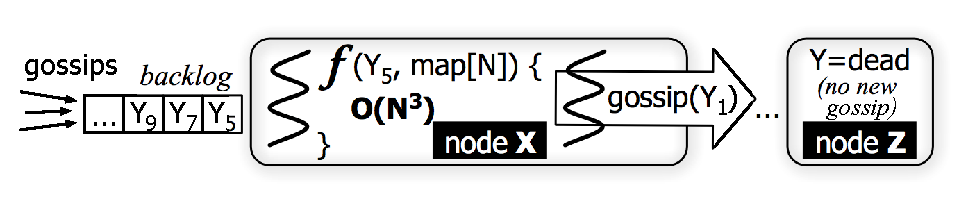
\includegraphics[height=0.8in]{F/cass1.eps}
%\includegraphics[height=0.6in]{F/empty.eps}
}
\vminfive
\mycaption[The problem of gossip-based failure detection in
Cassandra]{fig-cass1}{The problem of gossip-based failure detection in
Cassandra}{}
\vminfive
\end{figure}



To understand this bug, we need to understand the following protocols.
\begin{itemize}
\item {\bf Bootstrap:} Each node first creates partition keys (\eg, 32
random numbers) and gossips this information to peer nodes.
\item {\bf Gossip broadcast:} {\em Every second}, each node gossips to one 
random node about a list of nodes and partitions it knows (including
itself) and their {\em version} numbers.  Each node also increments its 
version number (``I'm still alive'') before gossiping.
\item {\bf Gossip processing:} The receiving node then finds any state
(metadata) differences between the two nodes to synchronize their views of
the ring.  Eventually, all nodes know about each other.
\item {\bf Failure detection:} {\em Every second}, a failure detection
daemon runs \cite{Lakshman+09-Cassandra}.  Put simply, if a node X has not 
received a new gossip about Y {\em from anyone} (Y's version has not 
changed after some period of time), X will declare Y dead (a flap).  When
X receives a new gossip about Y, it marks Y alive.
\end{itemize}

% about the bug
There are two factors that induce the bug.  The first is the {\em long latency
of scale-dependent state-update gossip processing during bootstrapping} (``f''
in Figure \ref{fig-cass1}).  While gossip processing is usually fast in a stable
cluster, it is expensive during bootstrapping as the gossips carry many new
state changes about the ring; the state-update processing time is
scale-dependent ($O(N^3)$); the larger the cluster ($N$), the larger the ring
map, the longer the processing time is.
%
This long latency is caused by {\bf (1)} state-update checkpoint to on-disk
database and {\bf (2)} multi-map cloning and updates.
%
The first one is needed for fast fault tolerance; after a node crashes, it can
reboot fast as it knows the latest view of the ring.
%
The second one is preferred for simplicity; Cassandra clones its \ts{MultiMap}
ring table and applies changes one by one to alleviate long write locks.
%
% in order to prevent a long write lock on the ring table which can block other
% user-facing protocols.

% long
The second factor is the {\em single threaded} implementation of gossip
processing.  As shown in Figure \ref{fig-cass1},  this inability to process
multiple gossips/state updates concurrently (for the sake of preventing
concurrency bugs) creates a {\em backlog} of new gossips.  For example, in {\em
every second}, Y tells someone it's alive with increasing version number (\eg,
Y$_7$), but the receiving nodes are still busy processing state changes and only
forward Y's old version number (\eg, Y$_1$).  As Y's new gossip is not
propagated on time,  other nodes (\eg, Z) will mark Y as dead.  This happens to
all nodes, not just Y.


\if 0
We mined bug repositories of four popular P2P key-value stores 
(Cassandra, Riak and 
Voldemort, Couchbase) and found \numStudy\footnote{The following are the 
  bugs we study (\textbf{with embedded hyperlinks}).
%
Cassandra: \caa, \cab, \cac, \cad, \cae ;
%
Couchbase: \cba, \cbb, \cbc, \cbd ;
%
Riak: \rka, \rkb ; and 
%
Voldemort: \vda.
%
This manual mining was arduous because there is no
standard jargon for ``scalability bugs'';
we might have missed other related bugs.
%
%For brevity, we only describe one bug in detail (\sec\ref{mot-bug})
%as the others have similar characteristics (\sec\ref{mot-observe}).
} control-plane scalability bugs.
%
These bugs caused significant availability problems such as long cluster
instability.
%
They also have complex characteristics (\sec\ref{mot-observe}).
\fi

\subsection{Observations}
\label{sec-scobs}

From the bug above, we make several important observations regarding
control-plane scalability bugs and distributed

\begin{itemize}
% only appear in large scale .. 
\item {\em Only appear at extreme scale:} \caone\ does not surface in 30-node
deployment. In 128-node cluster, the symptom appears mildly (tens of flaps).
From 200-500 nodes, flapping skyrockets to thousands of flaps. Testing in
small/medium scales is not sufficient.

% theory is not enough
\item {\em Scalable in design, but not in practice.}  Related to \caone, the
accrual failure detector \cite{Hayashibara+04-PhiFailureDetector} in
Cassandra is scalable in design \cite{Lakshman+09-Cassandra}.  However, the
design proof does not account gossip processing time, which can be long. To
understand the bug, the developers tried to ``do the [simple] math''
\cite{CA-One} but failed. In practice, new gossips are not propagated every
second (due to the backlog). The actual implementations overload gossips with
many other purposes (\eg, announcing boot/rebalance changes) beyond their
original design sketch.


% deep
\item {\em Implementation specific and hard to predict.}  The
backlog-induced flapping in \caone\ was caused specifically by Cassandra's
implementation choice: metadata checkpoint, multi-map cloning, and its
single-threaded implementation.  State-update processing time is hard to
predict (ranges from 0.001 to 4 seconds) as it depends on a 2-dimensional
input: the receiving node's ring table size and the number of new
state changes (\sec\ref{sec-eval}).

% not independent
\item {\em Cascading impacts of ``not-so-independent'' nodes.}  In
cluster-wide control protocols, distributed nodes are  not
necessarily independent; nodes must communicate with each other
to synchronize their views of cluster metadata.  As the cluster grows, the
cluster metadata size increases.  Thus, unpredictable processing time in
individual nodes can create cascading impacts to the whole cluster.

% 
\item {\em Long and difficult large-scale debugging:}
%
The bug report of \caone\ generated over 40 back-and-forth discussion
comments and took 2 months to fix.  It is apparent \cite{CA-One} that
there were many hurdles of deploying and debugging the buggy protocol at
real scale.  Important to note is that debugging is {\em not} a single
iteration; developers must {\em repeatedly} instrument the system (add
more logs) and re-run the system at scale to find and fix the bug, which
is not trivial.  The scalability bugs we studied took 6 to 157 days to
fix (27 on average).

\item {\em Not all developers have large test budgets:}
%
Another factor of delayed fixes is the lack of budget for large
test clusters.  Such luxury tends to be accessible to developers
in large companies, but not to
open-source developers.  When
\caone\ was submitted by a customer who had hundreds of nodes, the
Cassandra developers did not have an instant access to a test cluster of
the same scale.

% repeated 
\item {\em Quick fixes and repeated bugs:} Bugs are often fixed with quick
patches (development pressures), but the fix might not eradicate the problem
completely \cite{Yin+11-FixesBecomeBugs}.
%
The patch for \caone\ simply disables failure detection during bootstrap. But
the bug still appeared in another workload (\eg, scaling out from 128 to 256
nodes).
%
The simple fix has been removed later and the gossip protocol has been
redesigned.
%
And old fixes can become obsolete in protocol re-designs, which then can give
birth to new scalability bugs such as the fix for \csb{3831} became obsolete as
``vnodes'' was introduced, then led to a new scalability bug (\csb{3881}).

\end{itemize}

\subsection{State of the Art}

We now discuss popular approaches (simulation, extrapolation, and emulation) for
unearthing scalability bugs.
% ......
First, simulation approaches test system/application models in different scales
\cite{Calotoiu+13-ApmScaleBug, Laguna+15-DebugAtScale}. A model can look
scalable but the actual implementation can contain unforeseen bugs. Our
observations above accentuate the need for scale-checking distributed system
{\em implementations} at {\em real scale}.


% --------------- mini cluster
Second, extrapolation monitors system behaviors in ``mini clusters'' and 
extrapolates them to larger scales (\sec2.1 in \cite{Wang+14-Exalt}).
However, mini clusters tend to be order(s) of magnitude smaller than real
deployments.
% (\sec2.2 in \cite{Leesatapornwongsa+14-Drill}).  
% Not all
% developers have the luxury of mini clusters (\eg, ``mini'' can imply
% hundreds nodes in large companies).  
Most importantly, system behaviors do not always extrapolate linearly
\cite{Wang+14-Exalt}; for the bugs in our work (\sec\ref{sec-eval}), even an
extrapolation based on a 100-node cluster will not reveal the bug symptoms.

% --------------- emulation
Finally, real-scale emulation checks real implementations in an emulated
environment (\eg, DieCast and Exalt).
%
DieCast \cite{Gupta+08-DieCast}, invented for network emulation, can 
colocate many processes/VMs on a single machine as if they run 
individually without contention.  The trick is adding ``time dilation
factor'' (TDF) support \cite{Gupta+06-TimeDilation} into the VMM (\eg, Xen).
%
For example, TDF=5 implies that for every second of wall-clock time, each
emulated VM on the VMM believes that time has advanced by only 200 ms. 
%
The most significant drawback of DieCast is that high colocation factor
(\eg, TDF$=$100) is likely not desirable, for two reasons: prolonged
testing time (TDF$=$100 implies 100x longer run) and memory overcapacity.
%
Many distributed systems today are implemented in managed languages (\eg, Java,
Erlang) whose runtimes consume non-negligible memory overhead. Java and Erlang
VMs for example use around 70 and 64 MB of memory per process respectively. 
%
DieCast was only evaluated with TDF=10.

% co-location -- data compression -- exalt
Exalt \cite{Wang+14-Exalt} targets I/O-intensive scalability bugs.  With a
custom data compression, users' data is compressed to zero byte on disk (but the
size is recorded) while metadata is not compressed.  With this, Exalt can
co-locate 100 emulated HDFS datanodes on one machine.  In its evaluation, most
of the bugs reproduced are in the HDFS namenode which runs alone on one machine.
As the authors stated, their approach ``may not discover scalability problems
that arise at the nodes that are being emulated [the datanodes]'' (\sec4.1 in
\cite{Wang+14-Exalt}).  Thus, Exalt is not suitable for finding control-plane
scalability bugs in P2P distributed systems.

% P2P systems \cite{sosp01-past}.

% for control-plane
In summary, we did not find a fast single-machine approach that can scale-check
control-plane protocols in P2P systems.
%
The scalability bugs here are typically caused by the scale-dependent processing
time, not network or I/O bottlenecks.  As DieCast targets {\em network}
emulation via time dilation and Exalt targets {\em storage} space emulation via
compression, our work uniquely targets {\em processing time} emulation,
completing a missing piece.


\section{Conclusion}

In this chapter, we discuss about cloud-scale distributed systems, software
backend for the cloud computing. We show what the current trend of the systems
is and how they are design. We also discuss about distributed concurrency and
scalability, the two important aspects of cloud-scale distributed systems that
could threaten dependability of the systems. We briefly discuss how system
community address issues from the concurrency and scalability. Unfortunately,
distributed concurrency bugs are still an unsolved problem, and scalability bugs
are novel and not many works address about them.



\chapter{\taxdc: A Taxonomy of Non-Deterministic Concurrency Bugs in Cloud
Distributed Systems}

%\section{Introduction}
%\label{sec-intro}

Concurrency bugs are one notorious type of software bugs that happen in
concurrency systems. These timing-related bugs manifest non-deterministically,
and hence are extremely difficult to detect, diagnose, and fix. A huge body of
work exists in this space that focuses on ``local'' concurrency bugs (LC bugs)
in single-machine multi-threaded software, caused by incorrect interleaving of
memory accesses. And for cloud-scale distributed systems, the reliability is
also severely threatened by non-deterministic concurrency bugs as well, which
we refer as {\em distributed concurrency bugs} (DC bugs). Distributed systems
execute many complicated distributed protocols on hundreds/thousands of
machines with no common clocks, and must face a variety of random hardware
failures \cite{Do+13-Limplock, Gunawi+14-Cbs}. This combination makes
distributed systems prone to DC bugs caused by non-deterministic timing of
distributed events such as message arrivals, node crashes, reboots, and
timeouts. These DC bugs cannot be directly tackled by LC bug techniques, and
they cause fatal implications such as operation failures, downtimes, data loss
and inconsistencies.

Fighting DC bugs is challenging, particularly given the preliminary
understanding of real-world DC bugs.  To make progress, a comprehensive bug
study is needed. Past studies have closely examined bugs in various software
systems \cite{Chou+01-Empirical, Lu+13-FsEvolution, linux.asplos11}, which have
motivated and guided many aspects of reliability research.
%
There are few bug studies on cloud-scale distributed systems
\cite{Gunawi+14-Cbs, Li+13-ScopeBugStudy}, but they did not specifically dissect
DC bugs. There was an internal bug study dissecting network-failure-related DC
bugs to be a foundation to combat those bugs, but it was not published
\cite{Joshi+13-SetsudoTesting}, and one recent work analyzed non-determinism in
MapReduce programs but only discussed five bugs \cite{Xiao+14-NonDetMR}.
%
Thorough studies have also been conducted for LC bugs \cite{study.dsn10,
Lu+08-ConcurrencyBugStudy} with many follow-up work to date, yet {\em there is
no comprehensive study on real-world distributed concurrency bugs}. 

In this chapter, we fill the void by presenting our in-depth analysis of
real-world DC bugs in well-known cloud distributed systems, and introducing
\taxdc, the largest comprehensive taxonomy of DC bugs that covers several axes.
We briefly give an overview of \taxdc\ in Section \ref{sec-taxdc}, and present
our analysis in Section \ref{sec-trig}-\ref{sec-stat}.

\if 0
We fill this void in this chapter by presenting our in-depth analysis of
\numDcBugs\ DC bugs.  The bugs came from four popular cloud distributed
systems: Cassandra \cite{CassandraWeb}, HBase \cite{HBaseWeb}, Hadoop MapReduce
\cite{HadoopWeb}, and ZooKeeper \cite{ZooKeeperWeb}.
%
We introduce \taxdc, a comprehensive taxonomy of real-world DC bugs across
several axes of analysis such as the triggering timing condition and input
preconditions, error and failure symptoms, and fix strategies, as shown in
detail in Table \ref{tab:tax}.
\fi


\section{TaxDC Contribution}

As the main contribution, \tdc\ will be the first large-scale DC-bug benchmark.
In the last six years, bug benchmarks for LC bugs have been released
\cite{Jalbert11-RADBench, jieyu}, but no large-scale benchmarks exist for DC
bugs.  Researchers who want to evaluate the effectiveness of existing or new
tools in combating DC bugs do not have a benchmark reference.  \tdc\ provides
researchers with more than 100 thoroughly taxonomized DC bugs to choose from.
Practitioners can also use \tdc\ to check whether their systems have similar
bugs.  The DC bugs we studied are considerably general, representing bugs in
popular types of distributed systems.

As a side contribution, \tdc\ can help open up new research directions.  In the
past, the lack of understanding of real-world DC bugs has hindered researchers
to innovate new ways to combat DC bugs.  The state of the art focuses on three
lines of research: monitoring and postmortem debugging \cite{Geels+07-Friday,
Liu+08-D3S, Liu+07-WiDS, Reynolds+06-Pip}, testing and model checking
\cite{Guo+11-Demeter, Killian+07-LifeDeathMaceMC, Leesatapornwongsa+14-Samc,
Simsa+10-Dbug, Yang+09-Modist}, and verifiable language frameworks
\cite{Desai+13-PLang, Wilcox+15-Verdi}.  We hope our study will not only improve
these lines of research, but also inspire new research in bug detection tool
design, runtime prevention, and bug fixing, as elaborated more in Section
\ref{sec-less}.




\section{Methodology}
\label{sec-met}

%\myquote{``I'm suspecting there is a race condition.'' --- \zk{1496}}


% -------------------------------------------------
\vfifteen
\subsection{Basic Definitions}
\label{met-def}

A {\em distributed concurrency (DC) bug} is a 
concurrency bug in distributed
systems caused by distributed events that can occur in
non-deterministic order.  An {\em event} can be a message arrival/sending, 
local computation, fault, and reboot.
%
A {\em local concurrency (LC) bug} is a 
concurrency bug that happens locally
within a node due to thread interleaving.
%
In our model, a {\em distributed system} is a collection of
shared-nothing nodes.  Each node can run multiple protocols in
multiple threads.
%


% -------------------------------------------------
\subsection{Target Systems and Dataset}
\label{met-data}


Our study examined bugs from four widely-deployed
open-source datacenter distributed
systems that represent a diverse set of system architectures: Hadoop
MapReduce (including Yarn) \cite{HadoopWeb} representing distributed
computing frameworks, HBase \cite{HBaseWeb} and Cassandra
\cite{CassandraWeb} representing distributed key-value stores (also
known as NoSQL systems), and ZooKeeper \cite{ZooKeeperWeb}
representing synchronization services.
%
They are all fully complete systems containing many complex concurrent
protocols.  Throughout the chapter, we will present short examples of DC
bugs in these systems.  Some detailed examples are illustrated in Figure
\ref{fig-zook}, \ref{fig-paxos} and \ref{fig-hbase}.

The development projects of our target systems are all hosted under
Apache Software Foundation wherein organized issue repositories (named
``JIRA'') are maintained.  To date, across the four systems, there are
over 30,000 issues submitted.  One major challenge is that issues
pertaining to DC bugs do not always contain plain terms such as
``concurrency'', ``race'', ``atomicity'', \etc\ Scanning all the
issues is a daunting task.  Thus, we started our study from an open
source cloud bug study (CBS) database \cite{CBSWeb}, which already
labels issues related to concurrency bugs.  However, beyond simple
labeling, the CBS work did not differentiate DC from LC bugs and did
not dissect DC bugs further.

From CBS, we first filtered out LC bugs, then exclude 
DC bugs that do not contain clear description, and finally
randomly picked \numDcBugs\ samples
from the remaining detailed DC bugs, specifically \numDcCA\
Cassandra, \numDcHB\ HBase, \numDcMR\ Hadoop MapReduce, and \numDcZK\
ZooKeeper DC bugs, reported in January 2011-2014 (the time range of
CBS work).  
We have seen much fewer clearly explained DC bugs in CBS from 
Cassandra and ZooKeeper than those from HBase and Hadoop MapReduce, which 
may be related to the fact that they are different types of distributed
systems.  For example,  ZooKeeper, as a
synchronization service, is quite robust as it is built on the
assumption of event asynchrony since day one. Cassandra was built on
eventual consistency, and thus did not have many complex transactions,
until recently when Cassandra adopts Paxos.  We still see new DC bugs
throughout 2014-2015 (some pointed to us by the developers); they can
be included into \tdc\ in the future.




% ---------------------------------
\subsection{Taxonomy}
\label{met-tax}


\definecolor{Gray}{gray}{0.75}
\begin{table}[!htb]
%\footnotesize
\centering
\begin{tabular}{lp{5.5in}}
\toprule
%\rowcolor{Gray}
\multicolumn{2}{c}{{\bf Triggering} }\\
\midrule
\multicolumn{2}{l}{\it What is the triggering timing condition?}\\
&{Message arrives unexpectedly late/early}\\
&{Message arrives unexpectedly in the middle}\\
&{Fault (component failures) at an unexpected state}\\
&{Reboot at an unexpected state}\\
\multicolumn{2}{l}{\it What are the triggering inputs preconditions?}\\
 & {Fault, reboot, timeout, background protocols, and others}\\ 
%&{\scriptsize Node/Job crash}\\
%&{\scriptsize Node/Job restart after crash}\\
%&{\scriptsize Node/Job shut-down}\\
%&{\scriptsize Node/Job start-up}\\
%&{\scriptsize Time out}\\
%&{\scriptsize Others (e.g., client requests)}\\
\multicolumn{2}{l}{\it What is the triggering scope?}\\
&{\it How many nodes/messages/protocols are involved?}\\
\midrule
%\rowcolor{Gray}
\multicolumn{2}{c}{{\bf Errors \& Failures} }\\
\midrule
\multicolumn{2}{l}{\it What is the error symptom?}\\
&{Local memory exceptions}\\
&{Local semantic error messages \& exceptions}\\
&{Local hang}\\
&{Local silent errors (inconsistent local states) }\\
&{Global missing messages}\\
&{Global unexpected messages}\\
&{Global silent errors (inconsistent global states)}\\
\multicolumn{2}{l}{\it What is the failure symptom?}\\
&{Node downtimes, data loss/corruption, operation failures, slowdowns}\\
\midrule
%\rowcolor{Gray}
\multicolumn{2}{c}{{\bf Fixing} }\\
\midrule
\multicolumn{2}{l}{\it What is the fix strategy?}\\
&{Fix Timing: add global synchronization}\\
&{Fix Timing: add local synchronization}\\
&{Fix Handling: retry message handling at a later time}\\
&{Fix Handling: ignore a message}\\
&{Fix Handling: accepting a message without new computation logics}\\
&{Fix Handling: others}\\
\bottomrule
\end{tabular}
\mycaption[Taxonomy of DC Bugs]{tab:tax}{Taxonomy of DC Bugs}{}
\end{table}


We study the characteristics of DC
bugs along three key stages: triggering, errors \& failures, and
fixing (Table \ref{tab:tax}).
%
{\it Triggering} is the process where software execution states
deviate from correct to incorrect under specific conditions.  At the
end of this process, the manifestation of DC bugs changes from
non-deterministic to deterministic.
%
{\it Errors and failures} are internal and external software
misbehaviors.
%
{\it Fixing} shows how developers correct the bug.  We
will discuss in detail these categories in their respective sections.

% -----------------------------------------
\subsection{Threats to Validity}
\label{met-valid}

For every bug, we first ensure that the developers marked it as a real bug (not
a false positive).  We also check that the bug description is clear. Finally, We
then {\em re-enumerate} the full sequence of operations (the ``{\em steps}'') to
a clearer and more concise description such as the ones in Figure
\ref{fig-zook}. 
%
Our study cannot and does not cover DC bugs not fixed by the developers.  Even
for fixed bugs, we do not cover those that are not described clearly in the bug
repositories, a sacrifice we had to make to maintain the accuracy of our
results.  

Readers should be cautioned not to generalize the statistics we report as each
distributed system has unique purpose, design and implementation.
%
For example, we observe 2:1 overall ratio between order and atomicity violations
\sec\ref{trig-time}, however the individual ratios are different across the four
systems (\eg\ 1:2 in ZooKeeper and 6:1 in MapReduce).  
%
Like all empirical studies, our findings have to be interpreted with our
methodology in mind.

%\vfive % for good spacing

% -----------------------------------------
\subsection{TaxDC Database}
\label{met-db}

We name the product of our study \tdc\ database.  \tdc\ contains in
total \numTagsAll\ classification labels and \numDescLOC\ lines of
clear and concise re-description of the bugs (our version, that we
manually wrote) including the re-enumeration of the steps, triggering
conditions, errors and fixes.
%
We release \tdc\ to the public
\footnote{\url{http://ucare.cs.uchicago.edu/project/taxDC}}.  We believe \tdc\
will be a rich ``bug benchmark'' for researchers who want to tackle distributed
concurrency problems.  They will have sample bugs to begin with, advance their
work, and do not have to repeat our multi-people-year effort.


\vfive % for good spacing

% -----------------------------------------
\subsection{Detailed Terminologies}
\label{met-pres}

% ----------------- state
Below are the detailed terminologies we use in this chapter.
% basics
We use the term ``state'' to interchangeably imply {\em local state}
(both in-memory and on-disk per-node state) or {\em global state}
(a collection of local states and outstanding messages).
%
A {\em protocol} (\eg, read, write, load balancing) creates a chain of
events that modify system state.
%
User-facing protocols are referred as {\em foreground} protocols while
those generated by daemons or operators are referred
as {\em background} protocols.


% ------------------- fault
We consider four types of {\em events}: message, local computation,
fault and reboot.  The term {\em fault} represents component failures
such as crashes, timeouts, and disk errors.
%
A {\em timeout} (system-specific) implies a network disconnection
or busy peer node.
%
A {\em crash} usually implies the node experiences a power failure. %and does
%not come back up.
%
A {\em reboot} means the node comes back up.


% ---------------------------- DC bug presentation
Throughout the chapter, we present bug examples by abstracting
system-specific names.  As shown in Figure \ref{pat}, we use capital
letters for nodes (\eg, A, B), two small letters for a message between
two nodes (\mab\ is from A to B).  Occasionally, we attach
system-specific information in the subscript (\eg, A\sub{AppMaster}
sends \mab\sub{taskKill} message to B\sub{NodeManager}).
%
We use \underline{`` \textbf{/} ''} to imply concurrency
(\mac\ss\mbc\ implies the two messages can arrive at C in different
orders, \mac\ or \mbc\ first).
%
A dash, \underline{`` {\bf --} ''}, means causal relation of two
events (\mab-\mbc\ means \mab\ causally precedes\ \mbc).
%
Finally, we use \underline{``N{\bf *}''} to represent crash,
\underline{``N{\bf !}''} reboot, and \underline{``N{\bf +}''} local
computation at N.


% -------------------------- issue citation
We cite bug examples with clickable hyperlinks (\eg, \mr{3274}).
%
To keep most examples uniform, we use MapReduce examples whenever
possible.
%
%For interested readers, we cite more examples in the 
%footnotes (\eg, \spa\spb\spc).
%
%
We use the following abbreviations for system names:
``c/CA'' for Cassandra,
``h/HB'' for HBase, 
``m/MR'' for Hadoop MapReduce, and
``z/ZK'' for ZooKeeper;
% 
and for system-specific components:
``AM'' for application master,
``RM'' for resource manager,
``NM'' for node manager, 
``RS'' for region server, and
``ZAB'' for ZooKeeper atomic broadcast.



\section{Trigger}
\label{sec-trig}

DC bugs often have a long triggering process, with many local and
global events involved.  To better reason about this complicated process,
we study them from two
perspectives:

\begin{enumerate}

\item
{\em Timing conditions} (\sec\ref{trig-time}): For every DC bug, we
identify the smallest set of concurrent events $E$, so that a specific
ordering of $E$ can guarantee the bug manifestation.  This is similar
to the interleaving condition for LC bugs.



\item
{\em Input preconditions} (\sec\ref{trig-input}): In order for those
events in $E$ to happen, regardless of the ordering, certain inputs or
fault conditions (\eg, node crashes) must occur.  This is similar to the
input condition for LC bugs.

\end{enumerate}
%
Understanding the triggering can help the design of testing tools
that can proactively trigger DC bugs, bug detection tools that 
can predict which bugs can be triggered through program analysis,
and failure prevention tools that can  sabotage the triggering
conditions at run time.






% ===============================================
\subsection{Timing Conditions (TC)}
\label{trig-time}


Most DC bugs are triggered either by untimely delivery of messages,
referred to as {\it message timing bugs}, or by untimely faults or
reboots, referred to as {\it fault timing bugs}.  Rarely DC bugs are
triggered by both untimely messages and untimely faults, referred to
as {\it message-fault bugs}.  Table \ref{tab:trig} shows the
per-system breakdown and Figure \ref{bars}a (\BTMC) the overall
breakdown.  Since a few bugs are triggered by more than one type of
timing conditions
(\sec\ref{trig-scope}), the sum of numbers in Table \ref{tab:trig} is
slightly larger than the total number of DC bugs.

% ----------------------------
\paragraph{Message Timing Bugs.}

The timing conditions can be abstracted to two categories:


\begin{enumerate}[label=\alph*.]
%\begin{enumerate}

\item 
{\em Order violation} (\pctTrigOrder\ in Table \ref{tab:trig}) means 
a DC bug manifests
whenever a message comes earlier (later) than another event, which is
another message or a local computation, but not when the message comes
later (earlier).

\item
{\em Atomicity violation} (\pctTrigAtom\ in Table \ref{tab:trig}) 
means a DC bug manifests
whenever a message comes in the middle of a set of events, which is a
local computation or global communication, but not when the message
comes either before or after the events.

\end{enumerate}
%
LC and DC bugs are similar in that their timing conditions can both be
abstracted into the above two types. However, the subjects in these
conditions are different: shared memory accesses in LC and message
deliveries in DC. The ratio between order violation and atomicity
violation bugs are also different:
previous study of LC bugs showed that
atomicity violations are much more common than order violations in practice
%
\cite{Lu+08-ConcurrencyBugStudy}; 
our study of DC bugs 
shows that this relationship does not apply or even gets reversed
in several representative distributed systems.
%
%
%




\begin{table}[t]
\small
\centering
\begin{tabular}{lcccc}
\toprule
   & Ordering & Atomicity & Fault & Reboot \\
\midrule
CA &  4  & 4 & 6 & 5 \\
HB &  13  & 9 & 8 & 1 \\
MR & 25  & 4 & 5 & 3 \\
ZK &  4  & 8 & 7 & 5 \\
\midrule
All &  46  & 25 & 26 & 14 \\
\bottomrule
\end{tabular}

\mycaption[\#DC bugs triggered by timing conditions]{tab:trig}{\#DC bugs triggered by timing conditions}
{The total is more than \numDcBugs\ because some bugs
require more than one triggering condition. More specifically, 46 bugs 
(\pctTrigOrder) are caused {\em only} by 
ordering violations, 21 bugs (\pctTrigAtom) 
{\em only} by atomicity violations, and 4 bugs (\pctTrigMix) by multiple timing 
conditions (as also shown in Figure \ref{bars}a).}

\end{table}

 %----tab


\if 0
\jirafootnote{trig-time}{tab:trig}{
\spa \ca{5631}, \hb{4015}, \mr{3006}, \zk{1144};  % order violation
\spb \ca{1011}, \hb{4729}, \mr{5198}, \zk{1496};  % atomicity violation
\spc \ca{6415}, \hb{5806}, \mr{4819}, \zk{1653};  % crash timing
\spd \ca{2083}, \hb{6317}, \mr{5489}, \zk{975}.  % reboot timing
%
--- These examples are clickable hyperlinks pointing to 
\href{https://issues.apache.org/jira/browse/MAPREDUCE-3006}{https://issues.apache.org/jira/browse/S-NUM} where ``S'' and
``NUM'' are the system name and the issue number respectively.
For example, \mr{3006} points to 
\href{https://issues.apache.org/jira/browse/MAPREDUCE-3006}{https://issues.apache.org/jira/browse/MAPREDUCE-3006}.
}
\fi



% message-message
An order violation can originate from a race between two messages
({\em message-message race}) at one node.  The race can happen between
two message arrivals.  For example, Figure \ref{pat}a illustrates
\mac\ss\mbc\ race at node C in \mr{3274}.  Specifically, B\sub{RM}
sends to C\sub{NM} a task-init message (\mbc\sub{init}), and soon
afterwards, A\sub{AM} sends to C\sub{NM} a task-kill preemption
message (\mac\sub{kill}), however \mac\sub{kill} arrives {\em before}
\mbc\sub{init} and thus is incorrectly ignored by C.  The bug would
not manifest if \mac\sub{kill} arrives {\em after} \mbc\sub{init}
(Figure \ref{pat}b).
%
Message-message race can also happen between a message arrival and a
message sending.  For example, the \mab\ss\mbc\ race in Figure
\ref{pat}c depicts \hb{5780}.  In this bug, B\sub{RS} sends to
C\sub{Master} a cluster-join request (\mbc\sub{join}) unexpectedly
{\em before} a security-key message (\mab\sub{key}) from A\sub{ZK}
arrives at B, causing the initialization to abort.

Interestingly, message-message race can also occur concurrently across
two nodes.  For example, Figure \ref{pat}d illustrates
\mab\ss\mba\ race crisscrossing two nodes A and B in
\mr{5358}.  Specifically, A\sub{AM} sends \mab\sub{kill} to a backup
speculative task at B\sub{NM} because the job has completed, but
concurrently the backup task at B sends \mba\sub{complete} to A,
creating a double-complete exception at A.  If \mab\sub{kill} arrives
early at B, \mba\ will not exist and the bug will not manifest (Figure
\ref{pat}e).

% message-compute
An order violation can also originate from a race between a message
and a local computation ({\em message-compute race}).  For example,
Figure \ref{pat}f illustrates \mab\ss\lbp\ race in \mr{4157}.  First,
B\sub{AM} was informed that a task has finished and B plans to close
the job and remove its local temporary files (\lbp). However, just
{\em before} \lbp, A\sub{RM} sends to B a kill message (\mab) and
hence the files are never removed, eventually creating space issues.
To prevent the failure, the kill message has to arrive after the local
cleanup (Figure \ref{pat}g).


% atomicity violations
An atomicity violation, as defined above, originates when a message
arrives in the middle of a supposedly-atomic local computation or
global communication.
%
For example, Figure \ref{pat}h illustrates \mr{5009}.
When B\sub{NM}
is in the middle of a commit transaction, transferring task output
data (\mbc) to C\sub{HDFS},  A\sub{RM} sends a kill
preemption message (\mab) to B, preempting the task without resetting
commit states on C.
The system is never able to finish the commit --- when B
later reruns the task and tries to commit to C (\mbc'), C throws a
double-commit exception.  This failure would not happen if the kill
message (\mab) comes before or after the commit transaction
(\mbc).





\begin{figure}[t]

\centerline{
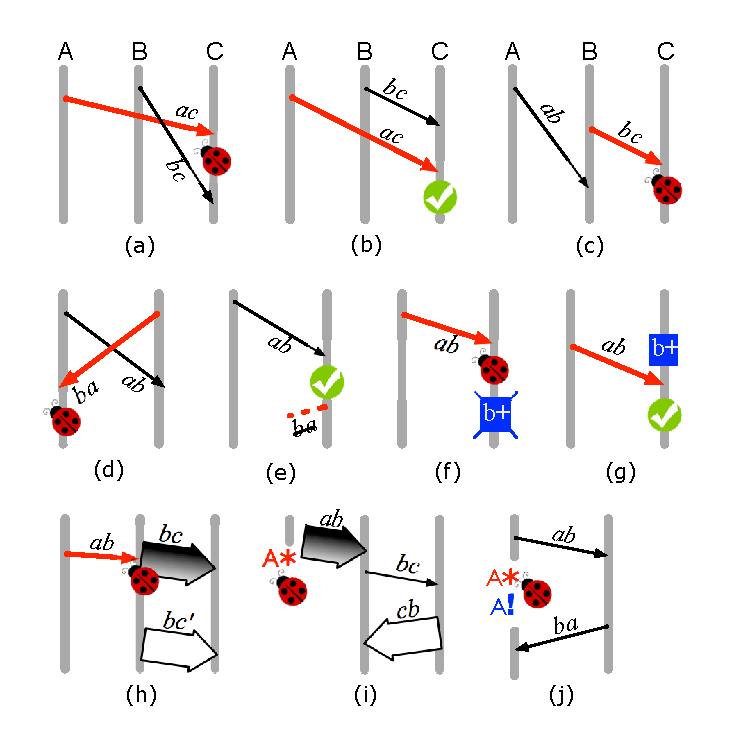
\includegraphics[width=3.5in]{F/patterns/basics.eps}
%\includegraphics[width=0.5\textwidth]{F/empty.eps}
}
\vminten
\mycaption[Triggering patterns]{pat}{Triggering patterns
(\sec{\ref{trig-time}})} {The three vertical lines represent the timeline of
nodes A, B and C.  An arrow with \ts{xy} label implies a message from X to Y.
A square box with label \ts{x+} implies a local state-modifying computation at
node X.  A thick arrow implies a set of messages performing an atomic
operation.  \ts{X*} and \ts{X!} implies a crash and reboot at node X
respectively (\sec\ref{met-pres}). All figures  are discussed in
\sec{\ref{trig-time}}}

\end{figure}



\if 0
\newtxt{The three lines represent
timeline of nodes A's, B's, and C's events (\ie\ sending/receiving
messages, local computations, crashes/reboots). Arrow lines ac mean
messages from A to C. Square boxes b+ mean local computations in B.
Thick arrows mean a set of messages doing an atomic operation. A*
means a crash of A, and A! means a reboot of A.  Figure (a)
illustrates an order violation pattern due to a race of two message
arrivals on node C (\ie\ messages ac/bc), which the bug would not
manifest if C receives the messages as in figure (b). Figures (c) and
(d) illustrate order violations between a message arrival and a
message sending (\ie\ ab/bc in (c), and ab/ba in (d)) which the bugs
would not happen if B receives the message ab before it sends a
message as in figure (e). Figure (f) illustrates an order violation
pattern between a message arrival and a local computation (\ie\ ab/b+)
which the bug would not manifest, if ab arrives after B has finished
b+ computation as in figure (g). Figure (h) illustrates an atomicity
violation that a message ab comes during B is doing an atomic
operation. Figure (i) illustrates a fault-timing pattern that A
crashes during an atomic operation (\ie\ A*/ab). Figure (j)
illustrates a reboot timing pattern that A crashes and reboots during
B processing a message ab, and A does not expect a message ba; the bug
would not happen if B tries to send ba and finds out A is dead. } }
\fi
 %----fig



% -------------------------
\paragraph{Fault and Reboot Timing Bugs.}

Fault and reboot timing bugs (\pctTrigFR\ in Table \ref{tab:trig})
manifest when faults and/or
reboots occur at specific global states $S$\sub{i}; the bugs do not
manifest if the faults and reboots happen at different global states
$S$\sub{j}. 

Figure \ref{pat}i illustrates a fault-timing bug in \mr{3858}.  Here,
A\sub{NM1} is sending a task's output to B\sub{AM} (\mab) but A
crashes in the middle (A*) leaving the output half-sent. 
The system is then unable to recover from this untimely crash --- B
detects the fault and reruns the task at C\sub{NM2} (via \mbc) and
later when C re-sends the output (\mcb), B throws an exception.  This
bug would not manifest, if the crash (A*) happens before/after
the output transfer (\mab).

Figure \ref{pat}j depicts a reboot-timing bug in \mr{3186}.  Here,
A\sub{RM} sends a job (\mab) to B\sub{AM} and while B is executing the
job, A crashes and reboots (A*, A!)  losing all its in-memory job
description.  Later, B sends a job-commit message (\mba) but A throws
an exception because A does not have the job information.  The bug
would not manifest if A reboots later: if A is still down when B sends
\mba\sub{commit} message, B will realize the crash and cancel the job before
A reboots and A will repeat the entire job assignment correctly.





\begin{figure}
\fbox{
\begin{minipage}{\textwidth}
\vspace{10pt}
\begin{quote}
{\bf \zk{1264}:}
\enumerate{
\item \fev{Follower F crashed} in the past,
\item \fev{F reboots} and joins the cluster; then \fev{F synchronizes data} with Leader L
\item F sends FOLLOWERINFO message to L [synchronization message]
\item L sends LEADERINFO message to F [synchronization message]
\item F sends ACKEPOCH message to L [synchronization message]
\item L sends SNAP message to F [synchronization message]
\item L sends data tree snapshot to F [synchronization message]
\item L sends NEWLEADER message to F [synchronization message]
\item \fev{Client C sends a request} to update data with Tx-\#15 to L; L does atomic broadcast to update all followers
\item L sends update proposal message for Tx-\#15 to F [broadcast message]
\item F sends update ack message for Tx-\#15 to L [broadcast message]
\item \fev{L sends update commit message} for Tx-\#15 to F [broadcast message]
\item \fev{F applies the update} for Tx-\#15 to in-memory data tree, but not to on-disk log (because F has not received UPTODATE message)
\item \fev{L sends UPTODATE message} to F [synchronization message]
\item C sends a request to update data with Tx-\#16 to L
\item L sends update proposal for Tx-\#16 to F
\item F sends update ack for Tx-\#16 to L
\item L sends update commit for Tx-\#16 to F
\item F applies the update for Tx-\#16 to in-memory data tree and on-disk log
\item \fev{F crashes} (before \fev{F does snapshot})
\item F reboots and joins the cluster again
\item L synchronized data with F by sending update starting from Tx-\#17
\item F loses the update for Tx-15 C did in step 9
}
\end{quote}
\vspace{10pt}
\end{minipage}
}
\mycaption{fig-taxdc-zk1264}{A DC bug in ZooKeeper}{This figure shows Figure
\ref{fig-zk1264} again. It shows a DC bug in ZooKeeper that is caused from a mix
of untimely message arrivals and crash timing. This bug surfaces when a follower
receives update commit messasge (step 12) in the middle of an atomic operation
(step 3-14) and the follower crashes before it does snapshot (step 20)}
\end{figure}



%\ev{(5)} L forwards the update request txid \#15 to F,

% ---------------------------------------------------- CA simple
% ---------------------------------------------------- CA complex
% ---------------------------------------------------- HBase simple
% ---------------------------------------------------- HBase complex
% ---------------------------------------------------- MR simple
% ---------------------------------------------------- MR complex
% ---------------------------------------------------- ZK simple
% ---------------------------------------------------- ZK complex




\paragraph{Message-Fault Bugs.}
Four DC bugs are caused by a combination of messages and faults. 
For example, in Figure
\ref{fig-taxdc-zk1264}, a message (step 12) arrives in the middle of some
atomic operation (step 3-14). This message atomicity violation leads
to an error that further requires a fault timing (step 20) to become an
externally visible failure.



\finding{DC bugs are triggered mostly by 
\textit{untimely messages} (\pctTrigMsg\ in Table \ref{tab:trig}) 
and % $\sim$70\%
sometimes by \textit{untimely faults/reboots} (\pctTrigFR), % $\sim$30\% 
and occasionally by a \textit{combination} of both (\pctTrigMix). % $<$5\%
Among untimely messages, two thirds commit order violations 
% Some untimely messages commit order violations (\pctTrigMsgOrder), %\sim$60
due to message-message or message-computation race on the node they arrive;
%(Figure\ref{pat}a--g);
the others commit atomicity violations.}
%(Figure\ref{pat}h).}

%These patterns provide
%important guidance to future research in combating DC bugs
%(\ref{sec-sol}).
%}




% ===============================================
\subsection{Input Preconditions (IP)} 
\label{trig-input}


The previous section presents simple timing conditions that can be
understood in few simple steps.  In practice, many of the conditions
happen ``deep'' in system execution.  In other words, the triggering
path is caused by complex input preconditions (IP) such as faults, reboots,
and multiple protocols.  Let's use the same example in Figure
\ref{fig-taxdc-zk1264}.
%
First, a fault and a reboot (step 1-2) and a client request (step 9)
must happen to create a path to the message atomicity violation (step
9 interfering with step 3-14).
%
Second, conflicting messages from two different protocols (ZAB and
NodeJoin initiated in step 2 and 9) have to follow specific
bug-triggering timing conditions.
%
Even after the atomicity violation (after step 14), the bug is not
guaranteed to lead to any error yet (\ie, a benign race).
%
Finally, the follower experiences an untimely fault (step 20), such
that after it reboots (step 21), a global replica-inconsistency error
will happen (step 23).
%
Put it in a reverse way, before step 20, the global state is $S$\sub{i}
and $S$\sub{i}$+$crash$\rightarrow$error, and the only way for the
system to reach $S$\sub{i} is from complex preconditions such as a
fault, a reboot, and some foreground and background protocols.



Statistically, Figure \ref{bars}b (\BFLT) shows that \pctFaultYes\ of
DC bugs must have at least one fault.  In more detail, Figure
\ref{bars}c-e (\BTO, \BCR, \BRB) shows the percentage of issues that
require timeouts, crashes and reboots respectively, including how many
instances of such faults must be there; the rest is other faults such
as disk errors (not shown).


Figure \ref{bars}f (\BPROT) shows how many ``protocol initiations''
mentioned in the bug description.  For example, if the system needs to
perform one execution of background protocol and also three concurrent
calls to the \ts{write} protocol, then we label it with four protocol
initiations.  Up to 3 protocol initiations covers three quarters of
DC bugs.
%
When we count the number of {\em unique} protocols involved in all the
bugs we study, we record \totProtCA\ Cassandra, \totProtHB\ HBase,
\totProtMR\ MapReduce, \totProtZK\ ZooKeeper unique protocols, or
\totProtAll\ protocols in total.  This again highlights the complexity
of fully complete systems.
%
Figure \ref{bars}g (\BBFG) shows our categorization of protocols that
are concurrently running into foreground only,
background only, and foreground-background (mix)
categories.  More than three quarters of the bugs involve some
background protocols and about a quarter involves a mix of foreground
and background protocols.

\finding{Many DC bugs need \textit{complex input preconditions}, 
such as faults
(\pctFaultYes\ in Figure \ref{bars}b), multiple protocols
(\pctProtMany\ in Figure \ref{bars}f), and background protocols 
(\pctProtBg\ in Figure \ref{bars}g) .}







\begin{figure}

\centerline{
\begin{tikzpicture}[font=\sffamily\footnotesize]
\begin{axis}[
xbar stacked,
y=0.8cm,
width=3.375in,
width=\columnwidth,
%height=120pt,
xmin=0,
xmax=100,
bar width=12pt,  
%xmajorgrids=true,
%ylabel={Categorizations},
%symbolic y coords={TRIG, CD, PIN, IMP, REP, EM, RB, CR, TO, FLT, LM, TSM, TSP, TSN},
symbolic y coords={REP, FIX, IMP, EM, ES, ERR, TSU, TSP, TSN, TSM, PIN, SP, RB, CR, TO, FLT, TRIG},
ytick=data,
%yticklabels={{(n) TRIG, (m) CD, (l) PIN, (k) IMP, (j) REP, (i) EM, (h) RB, (g) CR, (f) TO, (e) FLT, (d) LM, (c) TSM, (b) TSP, (a) TSN}},
yticklabels={{(q) WHR, (p) FIX, (o) FAIL, (n) ER-E/S, (m) ER-L/G, (l) ERROR, (k) TS-UEv, (j) TS-PR, (i) TS-ND, (h) TS-MSG, (g) IP-B/F, (f) IP-PR, (e) IP-RB, (d) IP-CR, (c) IP-TO, (b) IP-FLT, (a) TC}},
every axis y label/.style={at={(ticklabel cs:0.5)},rotate=90,anchor=near ticklabel},
xticklabels={,,},
axis x line*=none,
x axis line style={opacity=0},
axis y line*=right
]
\input{data-bars}
\end{tikzpicture}
%\includegraphics[width=1.8in]{F/empty.eps}
}
\vminten
\mycaption[Statistical overview of \tdc]{bars}{Statistical overview of \tdc}
{Timing Conditions (TC) is discussed in \sec\ref{trig-time},
Input Preconditions (IP) in \sec\ref{trig-input},
Triggering Scope (TS) in \sec\ref{trig-scope},
Errors (ER) in \sec\ref{err-err},
Failures (FAIL) in \sec\ref{err-fail},
Fixes (FIX) in \sec\ref{sec-fix},
and Where Found (WHR) in \sec\ref{sec-stat}.}
% \vten

\end{figure}


%
\if 0
nodes (TSN), 
protocols (TSP), 
background (BR), 
triggering messages (TSM), 
local-message race (LM), 
timeout (TO),
crashes (CR),
reboots (RB),
errorMessage (EM),
reported (REP),  
implication (IMP),
control/data plane (CDP), 
\fi



\begin{figure*}

\centerline{
%\includegraphics[width=6.5in]{F/empty.eps}
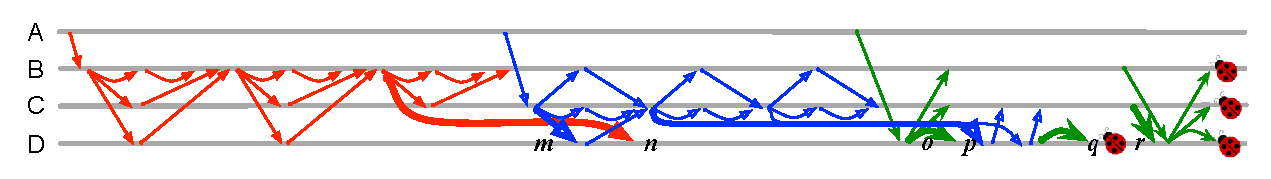
\includegraphics[width=7.0in]{F/paxos/paxos.eps}%
}
\vminfive
\mycaption[A Cassandra's Paxos bug]{fig-paxos}{A Cassandra's Paxos bug}{In \ca{6023}, 
three key-value updates 
(different arrow types)
concurrently execute the Paxos protocol on four nodes
(we simplify from the actual six nodes).
The bug requires three message-message race conditions:
(1) \emph{m} arrives before \emph{n}, 
(2) \emph{o} before \emph{p}, and
(3) \emph{q} before \emph{r}, which collectively
makes D corrupt the data and propagate the corruption
to all replicas after the last broadcast.
Note that the bug would not surface if any of the conditions
did not happen. 
It took us one full day to study this bug.
}
\vten
\end{figure*}

 % --

\if 0
\pctProtMany\ \xxx\ of the bugs must
have at least two different protocols running.  A protocol sometimes
must also be triggered multiple times (\eg, three clients concurrently
run the \ts{write} protocol), but currently we do not track this
number.  
\fi


\vten


% ===============================================
\subsection{Triggering Scope (TS)}
\label{trig-scope}


We now analyze the triggering scope (TS), which is a complexity measure of
DC-bug timing conditions.  We use four metrics to measure the scope:
message count (\BTSM), node (\BTSN), protocol (\BTSP), and untimely
event (\BTSU) counts as shown in Figure \ref{bars}h-k.  This statistic
is important with respect to the scalability of model checking, bug
detection and failure diagnostic tools
(\sec\ref{less-dmck}-\ref{less-diagnose}).

Message count implies the minimum
number of messages involved in $E$ as defined in the beginning of
section \ref{sec-trig}.  Figure \ref{bars}h (\BTSM) shows that one or two
triggering messages are the most common, with 7 messages as the
maximum.  Informally, zero implies fault timing bugs without any
message-related races, one implies message-compute race, two implies
message-message as in Figure \ref{pat}a, and three implies a scenario
such as \mac/(\mab-\mbc) race where \mab\ and \mac\ are concurrent or
non-blocking message sending operations.

The node and protocol scopes present how many nodes and protocols are
involved within the message scope.  Figure \ref{bars}i-j (\BTSN\ and
\BTSP) shows that the scale of node and protocol triggering scope is
also small, mostly two or three nodes and one or two protocols.

The untimely events count implies the total number of order
violations, atomicity violations, untimely faults and reboots in the
triggering timing condition of a bug.  Figure \ref{bars}k
(\BTSU) shows that only eight bugs require more than one untimely
events.  Four of them are message-fault bugs, each 
requiring one untimely message and one
untimely fault to trigger (\eg, step 9 and 20 in 
Figure \ref{fig-taxdc-zk1264}).  Three are fault-reboot timing bugs,
each requiring one untimely fault and one untimely reboot.
The last one is \ca{6023}, shown in Figure \ref{fig-paxos}, requiring
three message-message order violations to happen.

%TODO
% --- after the occurrence of 
%the one untimely event, the first error will deterministically propagate to
%failures

\finding{The \textit{timing conditions} of most DC bugs only involve 
\textit{one to three} messages, nodes, and protocols ($>$90\% in
Figure \ref{bars}h-j).  Most DC bugs are mostly triggered by 
only \textit{one} untimely event (\pctTrigScopeUnEvOne\ in Figure 
\ref{bars}k).}
%, which
%is a positive finding for the scalability of
%future bug finding tools (\sec\ref{less-bft}).
%Furthermore, more focus on interactions between foreground
%and background protocols that involve control logic should
%be exercised. 






\section{Errors and Failures}
\label{sec-err}

\subsection{Error Symptoms}
\label{err-err}

% goal
From the triggering conditions, we then scrutinize the {\em first}
error that happens immediately after.  First errors are the pivotal
point that bridges the triggering and error-propagation process.
Identifying first errors help failure diagnosis get closer to
disclosing bug triggering and root causes and help bug detection get
closer to accurately predict failures (\sec\ref{sec-less}).




% our category
We categorize first errors into {\em local} errors and {\em global}
errors, based on whether they can be observed from the triggering node
\nt\ alone.  Here, \nt\ is the node where triggering ends.  It is the
receiver node of untimely messages (\eg, node C in Figure \ref{pat}a)
or the node with untimely fault (\eg, node A in Figure \ref{pat}i).
For each error, we also check whether it is an {\it explicit} or {\em
  silent} error.  
Table \ref{tab:error} and Figure \ref{bars}l
(\BERR) show the per-system and overall breakdowns
respectively. 
Some MapReduce bugs caused multiple concurrent first errors of different types.

\if 0
\jirafootnote{err-err}{tab:error}{
\spa \ca{5925}, \hb{6375}, \mr{5198};  % local memory exception
\spb \hb{4540}, \mr{4607}, \zk{1046};           % local state machine/semantic
\spc \hb{5606}, \mr{4252}, \zk{1144};           % local hangs 
\spd \ca{2590}, \hb{6227}, \mr{4099}, \zk{1382};    % local silent (other than hang)
\spe \ca{1011}, \hb{4015}, \mr{2953};  % global wrong
\spf \ca{5393}, \hb{6060}, \mr{4819};  % global miss
\spg \ca{6023}, \hb{6070}, \zk{962}; % global silent
}
\fi


% local
First, DC bugs can manifest into both local explicit errors and local
silent errors. The former includes
%
{\em memory exceptions} such as null-pointer exceptions
(\pctErrLocMem\ in Table \ref{tab:error}) and {\em semantic errors} 
such as wrong state-machine transition exceptions thrown by 
the software (\pctErrLocSem).
%
Local silent errors include
%
{\em hangs}, such as forever waiting for certain states to change
or certain messages to arrive which are typically observed implicitly
by users (\pctErrLocHang),
%
and {\em local silent} state corruption, such as half-cleaned
temporary files (\pctErrLocSil).


\input{tab-error}

% global
When local error is non-obvious in \nt, we analyze if the error is
observable in other nodes communicating with \nt.  Many
DC bugs manifest into explicit global errors through {\em wrong
messages} (\pctErrGlobWrong\ in Table \ref{tab:error}). Specifically, 
the communicating
node receives an incorrect message from \nt, and throws an exception
during the message handling.  However, a few DC bugs still lead to
silent global errors. These include {\em missing messages}, where
\nt\ never sends a reply that the communicating node is waiting for
in the absence of timeout (\pctErrGlobMiss), and {\em global
  silent} state corruption such as replica inconsistencies
between \nt\ and the other nodes (\pctErrGlobSil).


\finding{\textit{Local} and \textit{global} first errors are about
equally common; \pctErrLoc\ vs. \pctErrGlob\ in Figure \ref{bars}m
(\BLG).  About half of the DC bugs generate \textit{explicit} first
errors (\pctErrExp), including local exceptions and global wrong
messages, and the remaining DC bugs lead to \textit{silent} errors
(\pctErrImp), as shown in Figure \ref{bars}n (\BES). 
%
Some of them immediately lead to hangs in the triggering node $N_T$
(\pctErrLocHang) or a node communicating with $N_T$
(\pctErrGlobMiss).  }








% =========================================
\subsection{Failure Symptoms}
\label{err-fail}






Figure \ref{bars}o (\BFAIL) shows that errors from DC bugs will
eventually lead to a wide range of fatal failures including
%
node downtimes (\pctFailNode),
data loss/corruption/inconsistencies (\pctFailData),
operation failures (\pctFailOp),
and performance degradation (\pctFailPer).
%
A node downtime happens when the node either crashes or
hangs (\ie, it may still be heartbeating).
It happens to both master/leader nodes and worker/follower nodes
in our study.
%Developers often have a hard
%time in debugging fail-silent behaviors and prefer fail-stop
%behaviors \cite{mr-3634}.
%
Data-related failures and performance problems are an artifact of
incorrect state logic induced from DC bugs.  For example, in HBase,
concurrent region updates and log splittings can cause data loss.
In Cassandra, some dead nodes are incorrectly listed as alive causing
unnecessary data movement that degrades performance.
% 
Node downtimes and data-related failures could also cause some operations
to fail.  To avoid double counting,
we consider a bug as causing operation failures only when it does not cause
node downtimes or data-related failures.

\if 0
\jirafootnotable{err-fail}{
\spa \hb{6153}, \mr{5198}, \zk{1144}; % node down
\spb \ca{2083}, \hb{6227}, \mr{4819}, \zk{1154}; % data loss / stale / corrupt
\spc \ca{5631}, \hb{5780}, \mr{4833}, \zk{1291}; % opfail
\spd \ca{3626}, \hb{5606}, \zk{975}; % perf degrade
}
\fi







\section{Fixes}
\label{sec-fix}

We next analyze bug patches to understand developers' fix strategies.
In general, we find that DC bugs can be fixed by either disabling the
triggering timing or changing the system's handling to that timing
({\em fix timing} vs. {\em fix handling}).  The former
prevents concurrency with extra synchronization and the latter allows
concurrency by handling untimely events properly.  Since message
timing bugs are fixed quite differently from fault timing bugs, we
separate them below.

% -------------------------------------------------
\subsection{Message Timing Bug Fixes}
\label{fix-msg}




The left half of Table \ref{tab:fix-msg} shows that
only one fifth of message timing bugs are fixed by disabling the
triggering timing, through either
 global or local synchronization.
%
Only a couple of bugs are fixed through extra {\em global
  synchronization}, mainly due to its complexity and communication
cost.  For example, to prevent a triggering pattern \lbp\ss\mab\ in
Figure \ref{pat}f, \mr{5465}'s fix {\em adds} a monitor on A\sub{RM}
to wait for \mba\sub{done} message from B\sub{AM} after B finishes
with its local computation (\lbp); the result is
\lbp-\mba-\mab\ global serialization.
%
More often, the buggy timing is disabled through {\em local
  synchronization}, such as re-ordering message sending operations
within a single node.  For example, \hb{5780}'s fix for
\mab\ss\mbc\ race in Figure \ref{pat}c forces the sending of
\mbc\ request at B to wait for the receipt of \mab; the result is
\mab-\mbc\ local serialization at B.




\begin{table}[t]
\small
\centering
\begin{tabular}{lccccccc}
\toprule
   & \multicolumn{2}{c}{Fix Timing} && \multicolumn{4}{c}{Fix Handling}\\
\cmidrule{2-3}
\cmidrule{5-8}
   & Glob & Loc & & Ret & Ign & Acc & Misc \\
\midrule
CA & 0   & 0 &&0 &1 & 3 & 4 \\
HB & 2   & 7 &&2 &1 & 7 & 3 \\
MR & 2   & 8 &&2 &7 & 8 & 3 \\
ZK & 0   & 4 &&0 &3 & 0 & 1 \\
\midrule
All& 4   & 19&&4 &12& 18& 11\\
\bottomrule
\end{tabular}
\mycaption[Fix strategies for message timing bugs]{tab:fix-msg}{Fix strategies for message timing bugs}
{Some bugs require more than one fix strategy.}
\end{table}



\if 0
\jirafootnote{fix-msg}{tab:fix-msg}{
\spa \hb{4729}, \mr{5465};                       % FixMsgTimeGlobal
\spb \hb{5780}, \mr{4099}, \zk{1144};            % FixMsgTimeLocal
\spc \hb{8940}, \mr{3274};                       % FixMsgHandRetry
\spd \ca{2371}, \hb{6227}, \mr{4252}, \zk{1208}; % FixMsgHandIgnore
\spe \ca{6013}, \hb{6070}, \mr{4637};     % FixMsgHandAcc
\spf \ca{5631}, \hb{6537}, \mr{3858}, \zk{962};     % FixMsgHandOth
}
\fi

The right half of Table \ref{tab:fix-msg} shows that fix handling is
more popular.  Fix handling fortunately can be simple;  many fixes
do {\em not} introduce brand-new computation logic into
the system, which can be done in three ways.
% 
First, the fix can handle the untimely message by simply {\em
  retrying} it at a later time (as opposed to ignoring or
accepting it incorrectly).  For example, to handle \mbc\ss\mac\ race
in Figure \ref{pat}a, \mr{3274} retries the unexpectedly-early
\mac\sub{kill} message at a later time, right after the
to-be-killed task starts.
%
Second, the fix can simply {\em ignore} the message (as opposed
to accepting it incorrectly).  For example, to handle
\mab\ss\mba\ race in Figure \ref{pat}d, \mr{5358} simply ignores
the unexpectedly-late \mba\sub{finish} message that arrives after
A\sub{AM} sends an \mab\sub{kill} message.
%
Finally, the patch can simply {\em accept} the untimely message
by {\em re-using} existing handlers (as opposed to ignoring it or throwing
an error).  For example, \mr{2995}'s fix changes the node AM to accept
an unexpectedly-early expiration message using an existing
handler that was originally designed to accept the same message at a
later state of AM.  \mr{5198}'s fix handles the atomicity violation by
using an existing handler and simply cancels the atomicity violating
local operation.
%
The rest of the fix-handling cases require new computation
logic to fix bugs.




% -------------------------------------------------
\subsection{Fault/Reboot Timing Bug Fixes}
\label{fix-crash}






Table \ref{tab:fix-crash} summarizes fix strategies for fault/reboot
timing bugs.  Unlike message timing, only rare bugs can be fixed by
controlling the triggering timing either globally or
locally (\eg, by controlling the timing of the fault recovery
actions).  A prime example is an HBase cluster-wide restart scenario
(\hb{3596}).  Here, as A shuts down earlier, B assumes responsibility
of A's regions (via a region-takeover recovery protocol), but soon B
shuts down as well with the regions still locked in ZooKeeper and the
takeover cannot be resumed after restart.  The patch simply adds a
delay before a node starts region takeover so that it will likely get
forced down before the takeover starts.

\input{tab-taxdc-fixcr}

\if 0
\jirafootnote{fix-crash}{tab:fix-crash}{
\spa \ca{2083}, \mr{4832}; % FixFaultTimeGlobal
\spb \hb{3596}, \mr{5476}, \zk{1264}; % FixFaultTimeLocal
\spc \ca{5393}, \hb{6060}, \mr{3186}; % FixFaultHandTO
\spd \ca{2496}, \hb{6317}, \mr{5489}, \zk{1154}; % FixFaultHandMsg
\spe \hb{10090},\mr{3186}, \zk{1154}; % FixFaultHandCS
\spf \ca{2590}, \hb{3446}, \mr{2783}, \zk{1419}; % FixFaultHandOth
}
\fi

For the majority of fault timing bugs, their patches conduct two
tasks: (1) detect the local/global state inconsistency caused by the
fault and (2) repair/recover the inconsistency.  The former is
accomplished through timeouts, additional message
exchanges, or others (omitted from Table \ref{tab:fix-crash}).
The latter can be achieved by simply canceling
operations or adding new computation logic.


\finding{A \textit{small number of fix strategies} have 
fixed most DC bugs.  A few DC bugs are fixed by \textit{disabling} 
the triggering timing (\pctFixTime\ in Figure \ref{bars}p), 
occasionally through extra messages and mostly 
through local operation re-orderings.
Most DC bugs are fixed by better handling the triggering 
timing, most of which do not introduce new computation logic --- 
they \textit{ignore} or \textit{delay} messages,
\textit{re-use} existing handlers, and \textit{cancel} computation 
(\pctFixHandEasy).}
%Figure \ref{bars}p (\BFIX) summarizes the numbers above.}


\section{Root Causes}
\label{sec-root}

It is difficult to know for sure why many DC-bug triggering conditions
were not anticipated by the developers (\ie, the root causes).  In
this section, we postulate some possible and common misbeliefs behind
DC bugs.


\vni {\it ``One hop is faster than two hop.''}
% one hop vs. two hop
Some bugs manifest under scenario \mbc\ss(\mba-\mac), similar to Figure
\ref{pat}a.  Developers may assume that \mbc\ (one hop) should arrive
earlier than \mba-\mac\ (two hops), but
\mac\ can arrive earlier and hit a DC bug.


\vni {\it ``No hop is faster than one hop.''}
Some bugs manifest under
scenario \mba-(\lbp\ss\mab), similar to Figure \ref{pat}f.  Developers
may incorrectly expect \lbp\ (local computation with no hop) to always
finish before \mab\ arrives (one hop).  
% ex: \zk{1270}
% ...

\vni {\it ``Atomic blocks cannot be broken.''}
Developers might believe that ``atomic'' blocks (local or global
transactions) 
can only be broken unintentionally by some faults such as crashes.
However, we see a few cases where atomic blocks are broken inadvertently
by the system itself, specifically via untimely arrival of
kill/preemption messages in the middle of an atomic block.
More often, the system does not record
this interruption
and thus unconsciously leaves state changes half way.  Contrary, in
fault-induced interruption, some fault recovery protocol typically
will handle it.


\vni {\it ``Interactions between multiple protocols seem to be
  safe.''} In common cases, multiple protocols rarely interact, and
even when they do, non-deterministic DC bugs might not surface.  This can
be unwittingly treated as normally safe, but does not mean
completely safe.


\if 0
\jirafootnotable{sec-root}{
\spa \hb{5780}, \mr{3596};  % one hop faster than two hops
\spb \mr{3780}, \zk{1270};  % no hop faster than one hop
\spc \hb{7643}, \mr{5198};  % atomic block broken
\spd \hb{5179}, \mr{4751}, \zk{1046};  % unsafe multiple protocol
\spe \ca{6571}, \mr{5465}, \zk{1496};  % add more states
}
\fi


\vni {\it ``Enough states are maintained.''}  Untimely events can
unexpectedly corrupt system states and when this happens the system
does not have enough information to recollect what had happened in the
past, as not all event history is logged.  We observe that some fixes
add new in-memory/on-disk state variables to handle
untimely message and fault timings.






\if 0
% this one is actually very rare, so i exclude this
\vni {\it ``An earlier message will receive an earlier reply.''}  For
example, given \mcb-\mbc\ss\mca-\mac, developers may expect the first
message's reply (\mbc) to arrive earlier than second message's reply
(\mac), again similarly to Figure \ref{pat}b.  But the replies can
arrive out of order (\ref{pat}a).  

% this one has similar nature as one hop vs. 2 hop
% i exclude this unless we have space later
\vni {\it ``The message sent earlier will take effect earlier''} For
example, we discussed earlier that \mr{3274} is triggered by a
\mbc/\mac\ race, and the software cannot handle \mac\sub{kill} when it
arrives earlier than \mbc\sub{init}.  (Figure \ref{pat}a), In
fact, \mbc\sub{init} is caused by another message \mab\sub{init} that
leaves node A\sub{AM} a while before \mac\sub{kill} does, which may be
why developers assume \mbc\ will arrive before \mac\ at C.
%
\fi




\finding{Many DC bugs are related with a few common misconceptions 
that are unique to distributed systems.}







\section{Other Statistics}
\label{sec-stat}

% \input{fig-whisk}

\if 0
\jirafootnotable{sec-stat}{\spa \mr{3006}, 
\mr{3531}, \mr{3596}, \mr{3656}, \mr{3858}, \mr{4252}}
\fi

We now present other quantitative findings not included in
previous discussions.  We attempted to measure the complexity of DC
bugs using four metrics: (a) the number of ``re-enumerated steps'' as
informally defined in \sec\ref{met-valid}, (b) the patch LOC
including new test suites for the corresponding bug, (c) the time to
resolve (TTR), and (d) the number of discussion comments between the
bug submitter and developers.
%
The 25th percentile, median, and 75th percentile for the four metrics
are
%
(a) \stepTFP, \stepMed, and \stepSFP\ steps, 
%
(b) \locTFP, \locMed, and \locSFP\ LOC, 
%
(c) \ttrTFP, \ttrMed, and \ttrSFP\ days to resolve, 
%
(d) \commTFP, \commMed, and \commSFP\ comments.  

In terms of where the bugs were found, Figure \ref{bars}r (\BWHR)
highlights that \pctWhrField\ were found in deployment and
\pctWhrTest\ from failed unit tests.  The rest, \pctWhrNotDef, are not
defined (could be manually found or from deployment).  Some DC bugs
were reported from large-scale deployments such as executions of
thousands of tasks on hundreds of machines.%\spa


\vten

\section{Lessons Learned}
\label{sec-less}

We now discuss the lessons learned, implications to existing tools
and the opportunities for new research in combating DC bugs.  
Although many high-level
directions can be adopted from work on LC bugs, there are many
interesting challenges and opportunities unique to DC bugs.

% ===========================================================
\subsection{Fault Paths and Multi-Protocol Interactions}
\label{less-fault}


Individual protocols tend to be robust in general.  Only 18 DC bugs
occur in {\em individual} protocols {\em without} any input 
fault condition; only
8 of them are in foreground protocols.  On the other hand, a large
majority of DC bugs happen due to concurrent executions of multiple
protocols and/or different fault timings (Finding {\bf \#2}).
%
This has a tremendous implication to input testing: {\em all types of
  verification, testing, and analysis approaches must consider fault
  injections and multiple protocols as input conditions.}
%
Although recent work has paid attention to this
\cite{Gunawi+11-FateDestini, Joshi+11-PreFail, 
Yuan+14-SimpleTesting}, we emphasize
that all forms of faults (\sec\ref{met-pres}) must be exercised.


% ======================================================
\subsection{Distributed Systems Model Checkers}
\label{less-dmck}

Assuming the necessary input conditions are exercised, the next
question is: can we test different event re-orderings to hit the
triggering timing (\sec\ref{trig-time})?  This is the job of
distributed system model checkers (dmck), which are gaining popularity
recently \cite{Guo+11-Demeter, 
Killian+07-LifeDeathMaceMC,
  Leesatapornwongsa+14-Samc, Simsa+10-Dbug,
  Yang+09-Modist}.  Dmck works by intercepting distributed events and
permuting their ordering.  The more events included, the more
scalability issues will arise due to state-space explosion.
%
To date, {\em no dmck completely controls the timings of
  \underline{all} necessary events} that might contribute to the
triggering timing (Finding {\bf \#1}).  MaceMC
\cite{Killian+07-LifeDeathMaceMC} only reorders messages and network
disconnections.  MoDist \cite{Guo+11-Demeter} exercises timeouts and
Demeter \cite{Guo+11-Demeter} intercepts messages and local
computation but they do not explore different timing of multiple
crashes and reboots.  SAMC \cite{Leesatapornwongsa+14-Samc} exercises
multiple faults but does not support timeout and thread controls.
Also, none of the above include storage faults
or timing issues \cite{Hao+16-TailAtStore}.
%
Therefore, continued research on scalable exploration algorithms is
needed, specifically 
% to reduce the state-space explosion 
when {\em all} the necessary events need to be controlled.
This could be helped by DC bugs' triggering scope characteristics
(Finding {\bf \#3}), just like that in
LC model checkers \cite{madanpldi07}.


% ======================================================
\subsection{Domain-Specific Specifications}
\label{less-spec}

Now, assuming the necessary events are controlled, the next question
is: do we have the specification to judge the manifestation of a bug?  
This is a plague for many tools.  For example,
Demeter does not find new bugs \cite{Guo+11-Demeter} and SAMC
\cite{Leesatapornwongsa+14-Samc} finds two new bugs.
Conversations with the authors suggest that their target systems do
not deploy detailed specifications, and thus some bugs are left
uncaught.  Deploying generic ``textbook'' specifications (\eg, ``only
one leader exists'') does not help as they could lead to false
positives (\eg, ZooKeeper allows two leaders at a single point in
time).  Many research papers on specifications only deploy few of them
\cite{Gunawi+11-FateDestini, Liu+08-D3S, Reynolds+06-Pip}.
Developers also
bemoan the hard-to-debug fail-silent problems \mr{3634} and
prefer to see easier-to-debug fail-stop bugs.  
%

On the positive side, \pctErrExp\ of DC bugs lead to
explicit first errors (Finding {\bf \#4}), implying that sanity checks
already in software can be harnessed as 
specifications
(more in \sec\ref{less-det}). On the other side, compared to
single-machine systems, distributed systems are much more capable
of masking errors. Therefore, these error
specifications have to be used with caution to avoid false 
positives. Furthermore, 
\pctErrImp\ of DC bugs lead to silent first errors (Finding {\bf \#4}).
Many of them proceed to ``silent failures'', such as data loss,
node hangs, etc. Even if they become explicit
errors later, these explicit errors could be far away from the 
initial triggering conditions (\eg, Figure \ref{fig-paxos}).
In short, {\em no matter how sophisticated the tools are, they are
  ineffective without accurate specifications}.
%
This motivates the creation or inference of local specifications
that can show early errors or symptoms of DC bugs.


% ======================================================
\subsection{Bug Detection Tools}
\label{less-det}

%We emphasize that the state of the art solutions for dc bugs fall into
%three camps: testing and model checking \cite{x}, verifiable
%distributed system frameworks \cite{x}, postmortem monitoring and
%debugging \cite{x}.  

We now discuss bug detection tools, which are
unfortunately rare for DC bugs, although very popular for
LC bugs
%
\cite{pacer,
  flanagan09fasttrack, 
  satish.pldi14, 
  avio.asplos06, 
  madanpldi07,
  savage97eraser}.
%
Bug detection tools look for bugs that match specific patterns.  They
cannot provide bug-free proof, but can be efficient in discovering
bugs when guided by the right patterns.
Our study provides guidance and patterns that can be exploited by
future DC bug detection.

\paragraph{Generic detection framework.}

Finding {\bf \#1} implies that
detecting DC bugs, particularly message-timing DC bugs, should focus
on two key tasks: (1) obtaining timing specifications, including order
and atomicity specifications among messages and computation; and (2)
detecting violations to these specifications through dynamic or static
analysis.

\paragraph{Invariant-guided detection.}

Likely program invariants can be learned from program
behaviors, and used as specifications in bug detection
\cite{engler01bugs, daikon00, avio.asplos06}.
The key challenge is to design
simple and suitable 
invariant templates.  For example, ``function $F_1$ should
always follow $F_2$'' is a useful template for API-related semantic
bugs \cite{engler01bugs};
%``variable $v$ should only be accessed by instruction $i_1$ and $i_2$''
%is good for memory bugs 
%\cite{accmon}; 
``the atomicity of accesses $a_1$ and $a_2$ should never be violated''
is effective for LC bugs \cite{avio.asplos06}.
%
%
Finding {\bf \#1} about triggering timing and Finding
\#{\bf 4} about error patterns provide empirical evidence that these
templates can be effective for DC bugs: ``message $bc$ should
arrive at $C$ before message $ac$ ($ca$) arrives (leaves)''; 
``message $ab$
should never arrive in the middle of event $e$ on node $B$''; and
``message $ab$ should always be replied''.

\paragraph{Misconception-guided bug detection.}

Knowing programmers' misconceptions can help bug detectors
focus on specifications likely to be violated.  LC bug
researchers have leveraged misconceptions such as {\it ``two near-by
  reads of the same variable should return the same value''}
\cite{avio.asplos06} and {\it ``a condition checked to be true should
  remain true when used''} \cite{ifcon.hpca14}.
%
%
Finding {\bf \#6} reveals that DC-unique common misconceptions, such
as {\it ``a single hop is faster than double hops''}, 
{\it ``local computation is   faster than one-hop message''}, 
{\it ``atomic blocks cannot be broken''}
can help DC bug detection.


\paragraph{Error-guided bug detection.} 

Finding {\bf \#4} shows that many DC bugs lead to explicit
local/global errors, which implies that timing specifications for many
DC bugs can be inferred backward based on explicit errors.  For
example, program analysis may reveal that a state-machine exception
$e$ will arise whenever $C$ receives message $ac$ before $bc$, which
provides a timing specification ($ac$ arrives before $bc$)
whose violation leads to a {\it local error}; or, the analysis may
reveal that exception $e$ arises whenever node $B$ receives a message
$cb$ from node $C$ and $C$ only sends $cb$ when $ac$ arrives at
$C$ before $bc$, which provides a timing specification whose
violation leads to a {\it wrong-message global error}; and so on.  
\if 0
We
have also observed two specific errors that have each been encountered
by at least 10 DC bugs. 
One is type-state error, such as task state-machine exceptions
in MapReduce, znode state-machine exceptions in ZooKeeper,
etc.; the
other is resource-usage error, such as use before creation or use
after destroy.  Bug detection tools tailored for these errors
can be very accurate.
\fi



\paragraph{Software testing.}

Testing takes a quarter of all software development resources,
and is crucial in exposing bugs before code
release.  Although many testing techniques have been proposed for LC
bugs \cite{madan.asplos10,
ctrigger.asplos09, racefuzzer}, there have been few for
DC bugs \cite{jcute}.
%
%
Finding {\bf \#2} implies that test input design has to consider
faults, concurrent protocols, and background protocols. Finding \#{\bf
  3} implies that {\it pairwise testing}, which targets every pair of
message ordering, every pair of protocol interaction, and so on, will
work much more effectively than {\it all combination testing}, which
exercises all possible total orders and interactions of all
messages and all protocols.
%
For example, a large number of DC bugs (Figure \ref{bars}d-f) can be 
found with inputs of at most two protocols, crashes and reboots.


\vten % good spacing

% ======================================================
\subsection{Failure Diagnosis}
\label{less-diagnose}


Given failure symptoms, distributed systems developers have to reason 
about many nodes to figure out the triggering and root cause of 
a failure.
Our study provides guidance to this challenging process of
failure diagnosis.

\paragraph{Slicing/dependence analysis.} 

Identifying which instructions can affect the outcome of an
instruction $i$ is a widely used debugging technique for deterministic
sequential bugs.  However, it cannot scale to the whole distributed
systems, and hence is rarely used.
%
%
Finding {\bf \#3} indicates that most DC bugs have deterministic error
propagation; Finding {\bf \#4} shows that many DC bugs have their
errors propagate through missing or
wrong messages.  Therefore, per-node dependence analysis that can
quickly identify whether the generation of a local error depends on
any incoming messages would help DC bug failure diagnosis to get
closer and closer to where the triggering events happen.




\paragraph{Error logging.}  

Error logging is crucial in failure diagnosis. If the
first error of a DC bug is an explicit local error, the error log can
help developers quickly identify the triggering node and focus their
diagnosis on one node.
%
%
Finding {\bf \#4} unfortunately shows that only \pctErrLocExp\ of DC bugs
lead to explicit local errors. This finding motivates future
tool to help make more DC bugs lead to explicit local errors.


\paragraph{Statistical debugging.}

Comparing success-run traces with failure-run traces can help identify
failure predictors for semantic bugs \cite{liblit03} 
and concurrency bugs \cite{cci.oopsla10}
in single-machine software.  The key
design question is what type of program properties should be
compared between failure and success runs. For example, branch
outcomes are compared for diagnosing semantic bugs but not for LC bugs.
%
%
Finding {\bf \#1} and \#{\bf 3} about triggering timing conditions
provide guidance for applying this approach for DC bugs. We can
collect all message sending/arrival time at runtime, and then find
rare event orderings that lead to failures by contrasting them with
common ``healthy'' orderings (\eg, Figure \ref{pat}b happens 99.99\%
of the time while Figure \ref{pat}a happens 0.01\% of the time).
%
%
Of course, there are challenges. Finding \#{\bf 2} and \#{\bf 3}
show that many DC bugs come from the interactions of
many protocols. Thus, it is not sufficient to only log a chain of messages
originated from the same request, a common practice in request logging
\cite{Chow+14-Mysterymachine}.  Furthermore, some DC bugs are triggered by
message-computation ordering. Therefore, logging messages alone is
not sufficient.

\paragraph{Record and Replay.}

Debugging LC concurrency bugs with record and deterministic replay is
a popular approach \cite{quickrec.isca13,
  doubleplay.asplos11}.  However, such an approach has not permeated
practices in distributed systems debugging.  A ZooKeeper developer
pointed us to a fresh DC bug that causes a whole-cluster outage but
has not been fixed for months because the deployment logs do not
record enough information to replay the bug (\zk{2172}).  There has
been 9 back-and-forth log changes and attachments with 72 discussion
comments between the bug submitter and the developers.  More studies
are needed to understand the gap between record-replay challenges in
practice and the current state of the art \cite{Geels+06-Liblog,
  Liu+07-WiDS}.

\if 0
There needs to be more work in record and replay debugging for DC bugs
beyond the current state of the art which typically focuses on single
protocols The challenges are similar to the ones for statistical
debugging discussed above.
\fi

%Geels+07-Friday, 





\vten % good spacing

% ======================================================
\subsection{Failure Prevention and Fixing}
\label{less-runtime}


\paragraph{Runtime Prevention.}

The manifestation of 
concurrency bugs can sometimes be prevented by
injecting delays at runtime.  This technique has been successfully
deployed to prevent LC bugs based on their timing
conditions \cite{DeadlockImmunity, avisio,conair.asplos13}.
%
%
Finding {\bf \#1} shows that many DC bugs are triggered by untimely
messages and hence can potentially be prevented this way.  For
example, none of the bugs shown in Figure \ref{pat}a--h would happen
if we delay a message arrival/sending or local computation.  Of
course, different from LC bugs, some of these delays have to rely on a
network interposition layer; similar with LC bugs, some
delays may lead to hangs, and hence cannot be adopted.



\paragraph{Bug Fixing.}

Recent work automatically fixes LC bugs by inserting lock/unlock or
signal/wait to prohibit buggy timing \cite{cfix.osdi12,
  grail.fse14, wang.osdi08}.
%
%
Finding {\bf \#5} shows that the same philosophy is promising for
\pctFixTime\ of studied DC bugs. Our study 
shows that this approach has to be tweaked to focus on using global
messages (\eg, ACKs) or local operation re-ordering, instead of lock
or signal, to fix DC bugs.  Finding {\bf \#5} indicates that
\pctFixHandEasy\ of those DC bugs are fixed by shifting message handlers,
ignoring messages, and canceling computation, without adding new
computation logic.  This presents a unique opportunity for developing
new and more aggressive fixing techniques.


\vfive  % good spacing

% ===========================================================
\subsection{Distributed Transactions}
\label{less-tx}

\if 0
\jirafootnotable{less-tx}{
\spa \hb{4729}, \hb{4540}, \hb{4539}, \hb{4015}.
}
\fi



\begin{figure}
\bugbox{
%---------------------------------
{\bf \hb{9095}:}
\enumerate{
\item RS successfully OPENED region R,
\item RS notifies ZK that region R is OPENED,
\item ZK continues region R state msg to Master,
\item Master starts processing OPENED msg,
\item Meanwhile RS CLOSED region R (asked by Client),
\item RS notifies ZK that region R is CLOSED,
\item Master asks ZK to delete znode for region R,
\fev{concurrently racing with step 6!},
\item ZK deletes region R's znode,
\item Master never assigns region R to any RS.
\fev{R becomes an orphan!}
}
%---------------------------------
}
\mycaption[Race of HBase's messages to ZooKeeper]{fig-hbase}{Race of HBase's messages to ZooKeeper}{}
%\vten
\end{figure}



In the middle of our study, we ask ourselves: if DC bugs can be
theoretically solved by distributed transactions, why doesn't such
technique eliminate DC bugs in practice?  Our answers are:
%
first, the {\em actual implementations of theoretically-proven
  distributed transactions are not always correct}
(as also alluded in other work \cite{Burrows06-Chubby, Ongaro+14-Raft}).
For example, new
DC bugs continue to surface in complex distributed transactions such
as ZooKeeper's ZAB and Cassandra's Paxos as they are continuously
modified.
%
Second, {\em distributed transactions are only a subset of a full
  complete system}.  A prime example is the use of ZooKeeper in HBase
for coordinating and sharing states between HBase masters and region
servers.  Although ZooKeeper provides linearization of updates, HBase
must handle its concurrent operations to ZooKeeper,
for example, step 6 and 7 in Figure \ref{fig-hbase};
there are many other similar examples.%\spa.
%
Put simply, there are many protocols that do not use distributed
transactions, instead they use domain-specific finite state machines,
which should be tested more heavily.


Another approach to eliminate non-deterministic bugs in distributed
protocols is by building deterministic distributed systems.  However, the
technique is still in its infancy, at least in terms of the impact to
performance (\eg, an order of magnitude of overhead \cite{Hunt+13-DDOS}).




% ======================================================
\subsection{Verifiable Frameworks}
\label{less-others}

Recently there is a growing work on new programming language frameworks
for building verifiable distributed systems \cite{Desai+13-PLang,
Hawblitzel+15-IronFleet, Wilcox+15-Verdi}, but they typically focus on the
main protocols  and not the full system including
the background protocols.  One major challenge is that 
just for the basic read and write protocols,
the length of the
proofs can reach thousands of lines of code, potentially
larger than the protocol implementation.
Unfortunately, our study shows that the complex
interaction between foreground and background protocols can lead to DC
bugs.  Therefore, for complete real-world systems, verification of the
entire set of the protocols is needed.
%

\subsection{LC bugs vs. DC bugs}
\label{less-lcdc}
There are clearly similarities between LC bugs and DC bugs, as, 
by definition, they are both timing-related non-deterministic bugs.
Many DC bugs contain LC components:
untimely messages may lead to unsynchronized accesses from 
multiple threads or multiple event-handlers 
\cite{vechev.oopsla13,satish.pldi14} in a single machine.
It is probably not a surprise that atomicity violations
and order violations are two dominant triggering timing conditions
for both LC and DC bugs (Finding {\bf \#1}). 
Our observation of the small triggering scope of most DC bugs
(Finding {\bf \#3})
is similar with that for LC bugs, which may be related to the nature
of the bug sets ---
more complicated bugs may be more difficult to fix, and
hence less likely to be included in empirical studies. 

There are also many differences between LC bugs and DC bugs, as they originate
from different programming paradigms and execution
environments. For example, order violations are much more common in DC bugs
than those in LC bugs (Finding {\bf \#1}); faults and reboots are much 
more common in DC bugs than those in LC bugs (Finding {\bf \#2}); 
the diagnosis of many DC bugs will have to reason beyond one node, 
clearly different from that of LC bugs (Finding {\bf \#4});
the fix
strategies for DC bugs are very different from those of LC bugs, because
enforcing global synchronization is difficult (Finding {\bf \#5}).


% -----------------------------------------------
\section{Conclusion}

In this chapter, we have shown our in-depth study result on DC bugs and
introduce \taxdc, the largest and most comprehensive taxonomy of DC bugs. 
\taxdc categorizes DC bugs in three major aspects including triggering, error
and failure, and fix. This chapter show some complexity of DC bugs such as:

\begin{itemize}
% surface
\item We see a lack of effective testing, verification, and analysis tools to
detect DC bugs during development process.

% protocols
\item Many DC bugs hide in complex concurrent executions of {\em multiple}
protocols and not only user-facing foreground protocols, but also background and
operational.

% faults
\item Majority of DC bugs surface in the presence of hardware faults such as
machine crashes (and reboots), network delay and partition (timeouts), and disk
errors.  

% silent
\item Half of DC bugs lead to silent failures and hence are hard to debug in
production and reproduce offline.

\end{itemize}

% ---------------------------------------------

However, our results also bring fresh and positive insights:

\begin{itemize}
% trigger-shan
\item From the triggering patterns, we see opportunities to build DC bug
detection to focus on timing-specification inference and violation detection.

% err-shan
\item Half of DC bugs lead to {\em explicit} local or global errors which allow
inferring timing specifications based on local correctness specifications, in
the form of error checking already provided by developers.

%fix-shan
\item Most DC bugs are fixed through a small set of strategies and some are
simple which implies research opportunities for automated in-production fixing
for DC bugs.

% highlights
%\item Many other observations are made that enable us to analyze the gap between
%state-of-the-art tools and real-world DC bugs as well as between research in LC
%and DC bugs.

\end{itemize}

We believe that our observations in this chapter will be a foundation to help us
advance the state of the art to combat DC bugs.


\chapter{SAMC: Semantic-Aware Model Checking for Fast Discovery of DC bugs in Cloud Distributed Systems}

%State of the art does not help.

As we discuss in Section \ref{sec-bg-dmck}, a recent popular approach to unearth
DC bugs is adopting distributed system model cheker or dmck. However, due to the
complexity of DC bugs that we discussin Chapter \ref{chp-taxdc} (\eg,
interactions of multiple protocols, and various and multiple faults), the state
of the art of dmcks still cannot work effectively \xxx{cite Modist, dbug,
demeter, macemc}. We observe that the existing systematic reduction policies
cannot find bugs quickly, and cannot scale with the inclusion of fault events.

In this chapter, we discuss how to advance the state of the art by leveraging
semantic awareness to assist model checking, and introduce ``Semantic-Aware
Model Checking'' (SAMC), a white-box model checking approach that takes semantic
knowledge of how events (\eg, messages, crashes, and reboots) are processed by
the target system and incorporates that information in reduction policies. We
first discuss background of dmck and the state of the art in Section \ref{dmck}

%To show the intuition
%behind SAMC, we first give an example of a simple leader election protocol.
%Then, we present SAMC architecture and our four reduction policies.

\section{Semantic Awareness}

In a simple leader election protocol, every node broadcasts its vote to reach a
quorum and elect a leader.  Each node begins by voting for itself (\eg, \ntwo\
broadcasts \ts{vote=2}).  Each node receives vote broadcasts from other peers
and processes every vote with this simplified code segment below.  As depicted
in the code segment below, if an incoming vote is less than the node's current
vote, it is simply discarded.  If it is larger, the node changes its vote and
broadcasts the new vote.

\begin{alltt}
if (msg.vote < myVote) \{
  discard;
\} else \{
  myVote = msg.vote; broadcast(myVote);
\}
\end{alltt}

Let's assume \nfour\ with \ts{vote=4} is receiving three concurrent messages
with votes \ts{1}, \ts{2}, and \ts{3} from its peers.  Here, a dmck with a
black-box DPOR approach must perform 6 (3!) orderings (\ts{123}, \ts{132}, and
so on).  This is because a black-box DPOR does {\em not} know the {\em message
processing semantic} (\ie, how messages will be processed by the receiving
node).  Thus, a black-box DPOR must treat all of them as dependent
(\sec\ref{mot-state}); they must be re-ordered for soundness.  However, by
knowing the processing logic above, a dmck can soundly conclude that all
orderings will lead to the same state; all messages will be discarded by \nfour\
and its local state will not change.  Thus, a semantic-aware dmck can reduce the
6 redundant executions to just 1 execution.

The example above shows a scalability limitation of a black-box dmck.
Fortunately, simple semantic knowledge has a great potential in removing
redundant executions.  Furthermore, semantic knowledge can be incorporated on
top of sound model checking foundations such as DPOR and symmetry, as we
describe next.

\input{samc-arch}
\subsection{Semantic-Aware Reduction Policies}
\label{sam-pol}



We now present four semantic-aware reduction policies that enable us to
define fine-grained event dependency/independency and symmetry beyond
what black-box approaches can do.




% policies

\section{SAMC}

\subsection{Outline}

Hopefully, you get the intuition, and now let me show you the architecture of
SAMC

\subsection{SAMC Architecture}

Like other model checker.

SAMC intercepts all outstanding messages, suspend them, and decides the order in
which they will be released.

To reduce unnecessary re-orderings, SAMC is built on foundational techniques,
such dynamic partial order reduction (or DPOR) and symmetry.

On top of this, we build generic reduction policies such as local message
independence, .

But semantic awareness is about protocol-specific, so testers need to write
protocol-specific rules on top of the generic policies.

Now, let me describe the middle layer here.

\section{LMI}

\subsection{Local-Message Independence}

Lets begin with LMI.

It’s about detecting independence among local mes- sages in each individual
node, as I’ve explained ear- lier.

\subsection{Local-Message Independence}

As you have seen, discard pattern is one thing that help us.

We also find other generic patterns such as increment and constant update.
an example of increment pattern is a master that counts ack messages from
slaves.

You can see here, re-ordering ack messages don’t make us see a new state.

this pattern is common in quorum writes such as in zookeeper and cassandra.

so here we can write increment predicates that skip re-ordering of ack messages.

And there is also constant pattern that talk about in the paper.








\begin{figure}[t]

\centerline{
%\includegraphics[height=1.2in]{F/empty.eps}
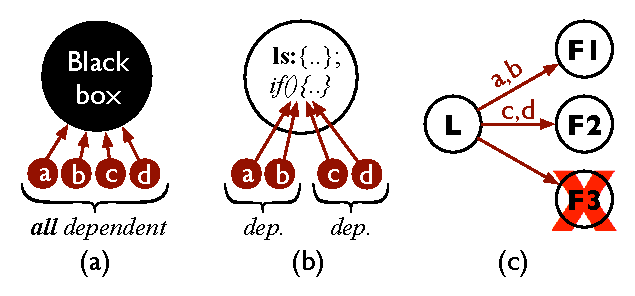
\includegraphics[height=2in]{F/pol/pol.eps}
}
\vminfive
\mycaption[LMI and CMI]{fig-pol}{LMI and CMI}{The figures
illustrate (a) a black-box approach, (b) local-message
independence with white-box knowledge, and (c)
crash-message independence.}
\vminten
\end{figure}





\subsubsection{Crash-Message Independence (CMI)}
\label{sam-cmi}


% CMI motivation
Figure~\ref{fig-pol}c illustrates the motivation behind our next
policy.  The figure resembles an atomic broadcast protocol where a
leader (\ts{L}) sends commit messages to the followers (\ts{F}s).
Let's assume commit messages \ts{ab} to \fone\ and \ts{cd} to \ftwo\
are still in flight (\ie, currently outstanding in the dmck; not
shown).  In addition, the dmck would like to crash \ftri, which we
label as a crash event \xx.  The question we raise is: how should \xx\
be re-ordered with respect to other outstanding messages
(\ma, \mb, \mc, and \md)?


% CMI problem dmck
As we mentioned before, we find {\em no} single dmck that incorporates
crash semantics into reduction policies.  As an implication, in our
example, the dmck must reorder \xx\ with respect to other outstanding
messages, generating executions \ts{Xabcd}, \ts{aXbcd}, \ts{abXcd},
and so on.  Worse, when \ts{abcd} are reordered, \xx\ will be
reordered again.  We find this as one major fundamental problem why
existing dmcks do not scale with the inclusion of failures.

% CMI pattern
To solve this, we introduce crash-message independence (CMI) which
defines {\em independency relationship between a to-be-injected crash
and outstanding messages}.  The key lies in these two crash reaction
patterns (global vs. local impact) running on the surviving nodes
(\eg, the leader node in Figure~\ref{fig-pol}c).


\begin{minipage}{\textwidth}
\begin{alltt}
\vfive
      \underline{Global impact:}       \underline{Local impact:}
      if (pg(X,ls))         if (pl(X,ls)) 
        modify(ls);           modify(ls);
        sendMsg();           
\end{alltt}
\vfive
\end{minipage}


% CMI pattern
The functions with prefix \pp\ are predicate functions that compare
the crash event \xx\ with respect to the surviving node's local state
(\eg, the leader's local state).  The \pg\ predicate in the {\em
global-impact} pattern defines that the crash \xx\ during the local
state \ls\ will lead to a local state change {\em and} new outgoing
messages (\eg, to other surviving nodes).  Here, no reduction can be
done because the new crash-induced outgoing messages must be
re-ordered with the current outstanding messages.  On the other hand,
reduction opportunities exist within the {\em local-impact} pattern,
wherein the \pl\ predicate specifies that the crash will just lead to
a local state change but not new messages, which implies that the
crash does not need to be re-ordered.  


% CMI policies
Based on the two crash impact patterns, we apply CMI in the following ways.
%
Given a local state \ls\ at node \nn, a peer failure \xx, and outstanding
messages (\mone...\mn) from \nn\ to other surviving peers, CMI performs:
%
(1) If \pl\ is true, then \xx\ and \mone...\mn\ are independent.
%
(2) If \pg\ is true, then \xx\ and \mone...\mn\ are dependent.
%
In Figure~\ref{fig-pol}c for example, if \pl\ is true in node \ts{L},
then \xx\ does not impact outstanding messages to \fone\ and \ftwo,
and thus \xx\ is independent to \ts{abcd}; exercising
\ts{Xabcd} is sufficient.


% CMI deployment
An example of CMI application is a quorum-based write protocol.  If a
follower crash occurs and quorum is still established, the leader will
just decrease the number of followers (local state change only).  Here,
for the protocol-specific rules, the tester can specify \pl\ with
\ts{\#follower} \ts{>=} \ts{majority} and \pg\ with the reverse. 
Overall, CMI helps dmck scale with the inclusion of failures, specifically by
skipping redundant re-orderings of crashes with respect to outstanding
messages.





% ---------------------------------
\subsection{Crash Recovery Symmetry (CRS)}
\label{sam-crs}


% RS Extra note
Before we discuss our next reduction policy, we emphasize again the
difference between message event and crash/reboot event.  Message
events are generated by the target system, and thus dmck can only
reduce the number of re-orderings (but it cannot reduce the events).
Contrary, crash events are generated by dmck, and thus there exists
opportunities to reduce the number of injected crashes.  For example,
in Figure~\ref{fig-pol}c, in addition to crashing \ftri, the dmck can
also crash \fone\ and \ftwo\ in different executions, but that might
not be necessary.

\input{code-crash}

% intuition: no individual node Ids, recovery depends on different states
To omit redundant crashes, we develop crash recovery symmetry (CRS).
The intuition is that some crashes often lead to symmetrical recovery
behaviors.  For example, let's assume a 4-node system with node
roles \ts{FFFL}.  At this state, crashing the first or second or third
node perhaps lead to the same recovery since all of them are
followers, and thereby injecting one follower crash could be enough.
Further on, if the system enters a slightly different
state, \ts{FFLF}, crashing any of the followers might give the same
result as above.  However, crashing the leader in the two cases
(\nfour\ in the first case and \ntri\ in the second) should perhaps be
treated differently because the recovery might involve the dead leader
ID.  The goal of CRS is to help dmck with crash decision.


% challenge
The main question in implementing CRS is: how to incorporate crash
recovery semantics into dmck?  Our solution is to compute {\em recovery
abstract global state} (\rags), a simple and concise representation of
crash recovery.  CRS builds \rags\ with the following steps:

First, we define that two recovery actions are symmetrical if they
produce the same messages and change the same local states in the same
way.

Second, we extract recovery logic from the code by flattening the
predicate-recovery pairs (\ie, recovery-related \ts{if} blocks).
Figure~\ref{code-crash} shows a simple example.  Different recovery
actions will be triggered based on which recovery predicate
(\prone, \prtwo, or \prtri) is true.  Each predicate depends on the
local state and the information about the crashing node.  Our key here
is to map each predicate-recovery pair to this formal pattern:


\vmintwo
{\small
\begin{alltt}
    if (\pri(ls, C.ls)) 
       modify(\ralsi); 
       \textit{(and/or)}
       sendMsg(\ralsi);
\end{alltt}
}
\vmintwo

Here, \pri\ is the recovery predicate for the i-th recovery action, and 
\ralsi\ is the recovery abstract local state 
(\ie, a subset of all fields of the local state involved in 
recovery).  That is, each recovery predicate defines what recovery
abstract local state that matters (\ie, \pri$\rightarrow$\{\ralsi\}).  For example, in Figure~\ref{code-crash},
if \prone\ is true, then \ralsone\ only contains the \ts{follower}
variable; if \prtri\ is true, \ralstri\ contains \ts{role}
and \ts{leaderId} variables.

Third, before we crash a node, we check which \pri\ will be true on
each surviving node and then obtain the \ralsi.  Next, we combine
\ralsi\ of all surviving nodes and {\em sort} them into a recovery
abstract global state (\rags);  sorting \rags\ helps us exploit
topological symmetry (\eg,  individual node IDs often do not matter).


Fourth, given a plan to crash a node, the algorithm above 
gives us the \rags\ that represents the corresponding recovery action.
We also maintain a history of \rags\ of previous injected crashes.
If the \rags\ already exists in the history, then the crash is skipped
because it will lead to a symmetrical recovery of the past.


% here here here
To recap with a concrete example, let's go back to the case
of \ts{FFFL} where we plan to enable crash(\none).  Based on the code
in Figure~\ref{code-crash}, the \rags\ is \{*, $\oslash$,
$\oslash$, \ts{\#follower=3}\}; 
* implies the crashing node, 
$\oslash$ means there is no true
predicate at the other two follower nodes, and \ts{\#follower=3} comes
from \ralsone\ of \prone\ of \nfour\ (the leader).  CRS will sort this
and check the history, and assuming no hit, then crash(\none) will be
enabled.  In another execution, SAMC finds that crash(\ntwo)
at \ts{FFFL} will lead to \rags:\{$\oslash$, *,
$\oslash$, \ts{\#follower=3}\}, which after sorting will hit the
history, and hence crash(\ntwo) is skipped.  If the system enters a
different state \ts{FFLF}, no follower crash will be injected, because
the \rags\ will be the same as above.  In terms of leader crash,
crashing the leader in the two cases will be treated differently
because in a leader crash, \prtri\ is true on followers and \prtri\
involves \ts{leaderId} which is different in the two cases.

% ...
In summary, the foundation of CRS is the computation of recovery
abstract global state (\rags) from the crash recovery logic extracted
from the target system via the \pri$\rightarrow$\{\ralsi\} pattern.
We believe this extraction method is simple because CRS does {\em not}
need to know the specifics of crash recovery; CRS just needs to know
what variables are involved in recovery (\ie, the \rals) .



\input{samc-rss}
\subsection{Pattern Extraction}
\label{sam-extract}


% summary
We have presented four general, simple, and powerful semantic-aware
reduction policies along with the generic event processing patterns.
With this, testers can write protocol-specific rules by extracting the
patterns from their target systems.  
%
Given the patterns described in previous sections, a tester must
perform what we call as ``extraction'' phase.  Here, the tester must
extract the patterns from the target system and write
protocol-specific rules specifically by filling in the predicates and
abstractions as defined in previous sections; in
Section~\ref{imp-targets}, we will show a real extraction result (\ie,
real rules).  Currently, the extraction phase is manual; we leave
automated approaches as a future work (\sec\ref{discuss}).
Nevertheless, we believe manual extraction is bearable for several
reasons.  First, today is the era of
DevOps~\cite{Limoncelli+11-Devops} where developers are testers and
vice versa; testers know the internals of their target systems.  This
is also largely true in cloud system development.  Second, the
processing patterns only cover high-level semantics; testers just fill
in the predicates and abstractions but no more details.  In fact,
simple semantics are enough to significantly help dmck go faster to
deeper states.






%\input{sam-ptop}
%\input{sam-pprio}



\subsection{Pattern Extraction}
\label{sam-extract}


% summary
We have presented four general, simple, and powerful semantic-aware
reduction policies along with the generic event processing patterns.
With this, testers can write protocol-specific rules by extracting the
patterns from their target systems.  
%
Given the patterns described in previous sections, a tester must
perform what we call as ``extraction'' phase.  Here, the tester must
extract the patterns from the target system and write
protocol-specific rules specifically by filling in the predicates and
abstractions as defined in previous sections; in
Section~\ref{imp-targets}, we will show a real extraction result (\ie,
real rules).  Currently, the extraction phase is manual; we leave
automated approaches as a future work (\sec\ref{discuss}).
Nevertheless, we believe manual extraction is bearable for several
reasons.  First, today is the era of
DevOps~\cite{Limoncelli+11-Devops} where developers are testers and
vice versa; testers know the internals of their target systems.  This
is also largely true in cloud system development.  Second, the
processing patterns only cover high-level semantics; testers just fill
in the predicates and abstractions but no more details.  In fact,
simple semantics are enough to significantly help dmck go faster to
deeper states.





\section{Implementation and Integration}
\label{sec-samc-impl}

In this section, we first describe our SAMC prototype, \sampro, which we
built from scratch because existing dmcks are either
proprietary~\cite{Yang+09-Modist} or only work on restricted high-level
languages (\eg, Mace~\cite{Killian+07-LifeDeathMaceMC}).  We will then describe
\sampro\ integration to three widely popular cloud systems,
ZooKeeper~\cite{Hunt+10-ZooKeeperPaper}, Hadoop/Yarn~\cite{Kumar+13-Yarn},
and Cassandra~\cite{Lakshman+09-Cassandra}.  Prior to \sampro, there was no
available dmck for these systems; they are still tested via unit tests, and
the test code size is bigger than the main code, but the tests are far from
reaching deep bugs.


\subsection{\sampro}
\label{imp-pro}

\sampro\ is written in \numLinesSamPro\ lines of code in Java, which
includes all the components mentioned in Section~\ref{mot-bgterms} and
Figure~\ref{fig-dmck}.  The detailed anatomy of dmck has been
thoroughly explained in literature~\cite{Guerraoui+11-McNoNetwork,
  Guo+11-Demeter, Killian+07-LifeDeathMaceMC, Simsa+10-Dbug,
  Yang+09-Modist}, and therefore for brevity, we will not discuss many
engineering details.  We will focus on SAMC-related parts.

% access source code
We design \sampro\ to be highly portable; we do not modify the target code
base significantly as we leverage a mature interposition technology,
AspectJ, for interposing network messages and timeouts.
% local state
Our interposition layer also sends local state information to the
\sampro\ server.
% crashes and reboots
\sampro\ is also equipped with crash and reboot scripts specific to the
target systems.  The tester can specify a budget of the maximum number of
crashes and reboots to inject per execution.
% summ
\sampro\ employs basic reduction mechanisms and advanced reduction policies
as described before.
% checks
We deploy safety checks at the server (\eg, no two leaders).  If a
check is violated, the trace that led to the bug is reported and 
can be deterministically replayed in \sampro.
% other supports
Overall, we have built all the necessary features to show the case of
SAMC.  Other features such as intra-node thread
interleavings~\cite{Guo+11-Demeter}, scale-out
parallelism~\cite{Simsa+12-ScalablePOR}, and virtual clock for network
delay~\cite{Yang+09-Modist} can be integrated to \sampro\ as well.


\vten % orphan text

\subsection{Integration to Target Systems}
\label{imp-targets}


In our work, the target systems are ZooKeeper, Hadoop 2.0/Yarn, and
Cassandra.  ZooKeeper~\cite{Hunt+10-ZooKeeperPaper} is a distributed
synchronization service acting as a backbone of many distributed systems
such as HBase and High-Availability HDFS.  Hadoop
2.0/Yarn~\cite{Kumar+13-Yarn} is the current generation of Hadoop that
separates cluster management and processing components.
Cassandra~\cite{Lakshman+09-Cassandra} is a distributed key-value store
derived from Amazon Dynamo~\cite{DeCandia+07-Dynamo}.

In total, we have model checked \numProtocols\ protocols: ZooKeeper
leader election (ZLE) and atomic broadcast (ZAB), Hadoop cluster
management (CM) and speculative execution (SE), and Cassandra
read/write (RW), hinted handoff (HH) and gossiper (GS).  These
protocols are highly asynchronous and thus susceptible to message
re-orderings and failures.

Table~\ref{tab-policies} shows a real sample of protocol-specific
rules that we wrote.  Rules are in general very short; we only wrote
\numLinesRule\ lines/protocol on average.  This shows the simplicity
of SAMC's integration to a wide variety of distributed system protocols.




\begin{sidewaystable*}[t]
\begin{center}
{\small
%---------------------------------
\begin{tabular}{p{1.9in}|p{2in}|p{2.1in}|p{2in}} 


\multicolumn{1}{c|}{{\bf Local-Message}} &
\multicolumn{1}{c|}{{\bf Crash-Message}} &
\multicolumn{1}{c|}{{\bf Crash Recovery}} &
\multicolumn{1}{c}{{\bf Reboot Synchronization}}
\\

\multicolumn{1}{c|}{{\bf Independence (LMI)}} &
\multicolumn{1}{c|}{{\bf Independence (CMI)}} &
\multicolumn{1}{c|}{{\bf Symmetry (CRS)}} &
\multicolumn{1}{c}{{\bf Symmetry (RSS)}}
\\


\hline  % =====================================================

% ----------------------------------------------- ZLE, LMI (1)

\vminten
{\footnotesize
\begin{alltt}
bool pd : !newVote(m, s);

bool pm : newVote(m, s);

bool newVote(m, s) : {
 if (m.ep > s.ep) 
   return true; 
 else if (m.ep == s.ep)
  if (m.tx > s.tx) 
   return true;
  else if (m.tx == s.tx &&
           m.lid > s.lid) 
   return true;
}
\end{alltt}
}

& % ----------------------------------------------- ZLE, CMI (1)

\vminten
{\footnotesize
\begin{alltt}
bool pg (s, X) : 
 if (s.rl == F && X.rl == L)
  return true;
 if (s.rl == L && X.rl == F
     && !quorumAfterX(s)
  return true;
 if (s.rl == S && X.rl == S) 
  return true;

bool pl (s, X) :
 if (s.rl == L && X.rl == F 
     && quorumAfterX(s)) 
  return true;

bool quorumAfterX(s) :
  ret ((s.fol-1) >= 
        s.all/2);
\end{alltt}
}

& % ----------------------------------------------- ZLE, CRS (1)

\vminten
{\footnotesize
\begin{alltt}
bool pr1(s,C):
 if (s.rl == L && C.rl == F
     && quorumAfterX(s))
  return true;
rals1:\{rl,fol,all\};

bool pr2(s,C):
 if (s.rl == L && C.rl == F 
     && !quorumAfterX(s))
 return true;
rals2: \{rl,fol,lid,ep,tx,clk\}

bool pr3(s,C):
 if (s.rl == F && c.rl == L)
  return true;
rals3: \{rl,fol,lid,ep,tx,clk\}

bool pr4:
 if (s.rl == S)
  return true;
rals4: \{rl,lid,ep,tx,clk\}
\end{alltt}
}


& % ----------------------------------------------- ZLE, RSS (1)

\vminten
{\footnotesize
\begin{alltt}
bool ps1(s,R):
 if (s.rl == L)
  return true;
sals1: \{rl,lid,ep,tx,clk\}

bool ps2(s,R):
 if (s.rl == F)
  return true;
sals2: \{rl,lid,ep,tx,clk\}

bool ps3(s,R):
 if (s.rl == S && 
     s.clk > R.clk)
  return true;
sals3: \{rl,lid,ep,tx,clk\}

bool ps4(s,R):
 if (s.rl == S && 
     moreUpdated(s, R))
  return true;
sals4: \{rl,lid,ep,tx,clk\}

bool moreUpdated(s, R):
 if (R.ep > s.ep)
  return true;
 else if (R.ep == s.ep)
  if (R.tx > s.tx) 
   return true;
  else if (R.tx == s.tx)
   if (R.lid > s.lid)
    return true;
\end{alltt}
}

\end{tabular}
}
%---------------------------------
\end{center}
%
\vminfive
\mycaption[Protocol-Specific Reduction Rules for ZLE]{tab-policies}{Protocol-Specific Reduction Rules for ZLE}{
%
The code above shows the actual protocol-specific rules for
ZLE protocol.  These rules are the inputs to the four reduction policies.
%
Many variables are abbreviated (ep: epoch, tx: latest
transaction ID, lid: leader ID, rl: role, fol: follower count, all: total
node count, clk: logical clock, L: leading, F: following, S: searching,
X/C: crashing node, R: rebooting node). LMI \pc\ and \pi\ predicates are not 
used for ZLE, but used for other protocols. 
%
}
%\vminfive
\end{sidewaystable*}


\if 0
zle-specific rule = 49
zab-specific rule = 33
mapreduce: 35 ..
protocol average = 
\fi



\input{samc-pro}
\input{samc-targets}

\section{Evaluation}

\subsection{Result}

We have built SAMC from scratch, and it took around 10,000 lines of code for all
mechanism.

We integrated to 7 protocols on 3 cloud systems, ZooKeeper, Cassandra,
MapReduce, including 10 version, new and old.

\subsection{Protocol-Specific Rules}

This is an example of protocol-specific rules from ZooKeeper leader election.

On average, it takes 35 lines of code for each protocols.

\subsection{Catching Old Bugs}

We can re-produce 12 old bugs that were reported by running SAMC with old
version of cloud systems.

We compare it with other state-of-the-art techniques, black-box DPOR that is
DPOR without domain-specific knowledge, random that is randomly re-ordering the
events, and random DPOR that is DPOR that start with random ordering.

Then we measure how many executions each model checker has to run until it reach
bugs.

By execution, I mean the ordering of events since the beginning up to
termination point or seeing some bugs.

This is SAMC.

This is black-box DPOR. This is random.

This is random DPOR.

5000+ means we have run 5000 executions but still not catch the bugs, and that
was around 2 days.

And here we compute speed-up.

Compare to black box, SAMC can do more than 94 times faster

And about 300 times faster compare to random and random DPOR.

\subsection{Reduction Ratio}

We also calculated reduction ratio compare to black- box DPOR on ZooKeeper
leader election protocol.

We also did fine-grained evaluation for each reduction policy too.

By trying different crashes and reboot, the result is shown in this table.

The reduction ratio increases when the number of crash and reboot increases. And
that means SAMC can find deep bugs faster than other techniques.

\subsection{Conclusion}

Today, we have cloud systems that quite complex, and deep bugs do happen to the
systems.

One approach to catch deep bugs is distributed system model checker, however,
the model checker treats the system as a black box and lead to state space
explosion

We are showing here that if we open the black box, make understanding of the
semantic, we can detect unnecessary ordering that lead to the same state, we
remove that and get one to two order of magnitude speedup

I believe that in the future we can use the principal of semantic awareness to
build more efficient reduction policies.



%\chapter{A Case of Scalability Bug in Cloud-Scale Distributed Systems}
\label{chp-scb}

In this and next chapter, we will discuss about ``scalability bugs'', a new
class of bugs that was born in an era of cloud computing, and how we can address
them. This chapter highlights an urgency in tackling scalability bugs by
studying deeply in \totAll\ scalability bugs from different popular scalable
distributed systems. Section \ref{scb} discusses motivation in tackling
scalability bugs and Section \ref{scb} gives some observations we gain from the
study.

\section{Motivation}

% scale, scale ... 
Is scale a friend or a foe \cite{Ousterhout+11-ScaleFriendEnemy}?
% CACM, is scale friend or enemy, john ousterhout
On the positive side, scale surpasses the limit of a single machine in
meeting users' increasing demands of compute and storage, which led to
many inventions of ``cloud-scale'' distributed systems
\cite{Chang+06-BigTable, 
DeanGhemawat04-MapReduce, 
DeCandia+07-Dynamo,
Ghemawat+03-GoogleFS, 
Hindman+11-Mesos,
Verma+15-Borg}.  The field has witnessed a
phenomenal deployment scale of such systems;
%
Netflix runs tens of 500-node Cassandra clusters \cite{RunningNetflix13},
% Running Netflix on Cassandra in the Cloud (youtube), Adriak Crockcroft
% https://www.youtube.com/watch?v=97VBdgIgcCU
Apple deploys a total of 100,000 Cassandra nodes \cite{WikiCassandra}, 
% https://en.wikipedia.org/wiki/Apache_Cassandra
and Yahoo! recently revealed the use of 40,000 Hadoop servers,
with a 4500-node cluster as the largest one \cite{LargestHadoop}.
% Http://www.techrepublic.com/article/why-the-worlds-largest-hadoop-installation-may-soon-become-the-norm/

% dark side, foe
On the negative side, scale creates new development and deployment issues.
Developers must ensure that their algorithms and protocol designs
to be scalable.
However, until real deployment takes place, unexpected bugs 
in the actual implementations are unforeseen.
% more and more
This new era of cloud-scale distributed systems has given birth
to a new type of bug: {\em scalability bugs}.  They are latent bugs that
are scale-dependent; they only surface in large-scale deployments, but not
in small/medium-scale ones.  Their presence jeopardizes systems
reliability and availability at scale.

As an example, let us consider a bug in Cassandra, a
highly-scalable peer-to-peer key-value store.  If a customer initially
deploys a cluster of 50 nodes and later scales it out with 50 additional
nodes, the operation can be done smoothly.  However, if the customer
deploys a 200-node cluster and then adds 200 more nodes, the protocol that
rebalances the key-range partitions (which nodes should own which key
ranges) becomes CPU intensive as the calculation has an $O(N^3)$
complexity where $N$ is the number of nodes.  This combined with the
gossiping and failure detection logic leads to a scalability bug that
makes the cluster unstable (many live nodes are declared as dead, making
some data not reachable by the users). We give full detail of the Cassandra bug
in Section \ref{scb}.

% example
We perform an in-depth study of
\totAll scalability bugs reported from the deployments
of popular large-scale systems such as
Hadoop,
HBase,
HDFS,
Cassandra,
Couchbase,
Riak, and
Voldemort.
%
From this study, we observed many challenges in finding, reproducing, and
debugging scalability bugs.
%
As in the example above, bug symptoms sometimes surface only in large
deployment scales (\eg, $N$$>$100 nodes), hence small/medium-scale testing
is not enough.  Yet, not all developers have large test budgets, and even
when they do, debugging on hundreds of nodes is time consuming and
difficult.
%
Furthermore, protocol algorithms can be scalable in the design sketches,
but not necessarily in the real deployments; there are specific
implementation details whose implications at scale are hard to predict. We
discuss more about our observations on scalability bugs in Section \ref{scb}.



\subsection{A Sample Bug (\caone)}
\label{mot-bug}

\begin{figure}

\centerline{
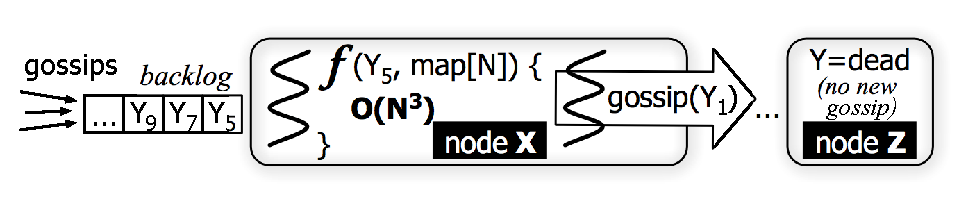
\includegraphics[height=0.8in]{F/cass1.eps}
%\includegraphics[height=0.6in]{F/empty.eps}
}
\vminfive
\mycaption[The problem of gossip-based failure detection in
Cassandra]{fig-cass1}{The problem of gossip-based failure detection in
Cassandra}{}
\vminfive
\end{figure}



We now describe in detail a control-plane scalability bug in
Cassandra, \ca{6127} \cite{CA-One}, 
% caone: jira link (see studies.tex)
which we use as a sample bug.
%
The bug surfaced on a cluster with hundreds of nodes and led to
``\textit{\textbf{flapping}}'' nodes, a condition where node up/down
status continuously changes;  tens of thousands of flaps\footnote{A 
``\textbf{flap}''
  is when a node X marks a peer node Y as down.}  were observed.




To understand this bug, we need to understand the following protocols.

\begin{enumerate}

\item {\bf Bootstrap:} Each node first creates partition keys (\eg, 32
random numbers) and gossips this information to peer nodes.
 
\item {\bf Gossip broadcast:} {\em Every second}, each node gossips to one
random node about a list of nodes and partitions it knows (including
itself) and their {\em version} numbers.  Each node also increments its
version number (``I'm still alive'') before gossiping.
 
\item {\bf Gossip processing:} The receiving node then finds any state
(metadata) differences between the two nodes to synchronize their views of
the ring.  Eventually, all nodes know about each other.
 
\item {\bf Failure detection:} {\em Every second}, a failure detection
daemon runs \cite{Lakshman+09-Cassandra}.  Put simply, if a node X has not
received a new gossip about Y {\em from anyone} (Y's version has not
changed after some period of time), X will declare Y dead (a flap).  When
X receives a new gossip about Y, it marks Y alive.

\end{enumerate}



% about the bug
There are two factors that induce the bug.  The
first is the {\em long latency of scale-dependent state-update gossip
  processing during bootstrapping} (``f'' in Figure \ref{fig-cass1}).  
While gossip processing is
usually fast in a stable cluster, it is expensive during bootstrapping as
the gossips carry many new state changes about the ring; the state-update
processing time is scale-dependent ($O(N^3)$); the larger the cluster ($N$), 
the larger the ring map, the longer the processing time is.
%
This long latency is caused by {\bf (1)} state-update checkpoint to on-disk
database and {\bf (2)} multi-map cloning and updates.
%
The first one is needed for fast fault tolerance; after a node crashes, it
can reboot fast as it knows the latest view of the ring.
%
The second one is preferred for simplicity; Cassandra clones its
\ts{MultiMap} ring table and applies changes one by one to alleviate 
long write locks.
%
% in order
% to prevent a long write lock on the ring table which can block other
% user-facing protocols.

% long
The second factor is the {\em single threaded} implementation of gossip
processing.  As shown in Figure \ref{fig-cass1},  this inability to process
multiple gossips/state updates concurrently 
(for the sake of preventing concurrency bugs) creates a {\em backlog} of new 
gossips.  For
example, in {\em every second}, Y tells someone it's alive with increasing
version number (\eg, Y$_7$), but the receiving nodes are still busy
processing state changes and only forward Y's old version number (\eg,
Y$_1$).  As Y's new gossip is not propagated on time,  other nodes
(\eg, Z) will mark Y as dead.  This happens to all
nodes, not just Y.





%http://docs.datastax.com/en/cql/3.1/cql/cql_intro_c.html


%


\section{Observations}
\label{mot-observe}

From the bug in previous section and all the bugs we studied, we make several
important observations.
%  regarding control-plane scalability bugs and distributed system designs.

\begin{itemize}
% only appear in large scale .. 
\item {\em Only appear at extreme scale:} \caone does not surface in 30-node
deployment.  In 128-node cluster, the symptom appears mildly (tens of
flaps).  From 200-500 nodes, flapping skyrockets from hundreds to 
thousands of flaps.  Testing in small/medium scales is not sufficient,
which is also true for other bugs we studied (\sec\ref{sec-eval}).





% theory is not enough
\item {\em Scalable in design, but not in practice.}  Related to \caone,
the accrual failure detector/gossiper
\cite{Hayashibara+04-PhiFailureDetector} was interestingly adopted by
Cassandra as it is scalable in design \cite{Lakshman+09-Cassandra}.
However, the design proof does not account gossip processing time during
bootstrap, which can be long.  To understand the bug, the developers tried
to ``do the [simple] math'' \cite{CA-One} but failed.  In practice, the
assumption that new gossips are propagated every second is not met (due to
the backlog).  The actual implementations overload gossips with many other
purposes (\eg, announcing boot/rebalance changes) beyond their original
design sketch.



% deep
\item {\em Implementation specific and hard to predict.}  The
backlog-induced flapping in \caone was caused specifically by Cassandra's
implementation choice: metadata checkpoint, multi-map cloning, and its
single-threaded implementation.  State-update processing time is hard to
predict (ranges from 0.001 to 4 seconds) as it depends on a 2-dimensional
input: the receiving node's ring table size and the number of new
state changes (\sec\ref{sec-eval}).

% a two-dimensional input; more in \sec\ref{sec-eval}).  

% not independent
\item {\em Cascading impacts of ``not-so-independent'' nodes.}  In 
cluster-wide control protocols, distributed nodes are  not
necessarily independent; nodes must communicate with each other
to synchronize their views of cluster metadata.  As the cluster grows, the
cluster metadata size increases.  Thus, unpredictable processing time in
individual nodes can create cascading impacts to the whole cluster.


% 
\item {\em Long and difficult large-scale debugging:} 
%
The bug report of \caone generated over 40 back-and-forth discussion
comments and took 2 months to fix.  It is apparent \cite{CA-One} that
there were many hurdles of deploying and debugging the buggy protocol at
real scale.  Important to note is that debugging is {\em not} a single
iteration; developers must {\em repeatedly} instrument the system (add
more logs) and re-run the system at scale to find and fix the bug, which
is not trivial.  The scalability bugs we studied took 6 to 157 days to
fix (27 on average).


\item {\em Not all developers have large test budgets:}
%
Another factor of delayed fixes is the lack of budget for large
test clusters.  Such luxury tends to be accessible to developers 
in large companies, but not to 
open-source developers.  When
\caone was submitted by a customer who had hundreds of nodes, the
Cassandra developers did not have an instant access to a test cluster of
the same scale.



% repeated 
\item {\em Quick fixes and repeated bugs:} Bugs are often fixed with quick
patches (development pressures), but the new fix might not eradicate the
problem completely \cite{Yin+11-FixesBecomeBugs}.
%
For example, for \caone, the patch simply disables failure detection during
bootstrap.  As the protocol was not redesigned, the bug still appeared in
another workload (\eg, scaling out from 128 to 256 nodes).
%
In the latest Cassandra, the simple fix has been removed and the gossip
protocol has been redesigned.
%
We also found that old fixes can become obsolete in 
protocol re-designs, which then can give birth to new scalability bugs. 
%
For example, the fix for \ca{3831} became obsolete as ``vnodes'' was
introduced, which then gave rise to a new 
vnode-related scalability bug
(\ca{3881}).
%
A scale-check could have ensured that new fixes remove old scalability bugs
entirely and similar bugs do not re-surface in new designs.
\end{itemize}


\if 0
Our observations above accentuate the need for scale-checking distributed
system {\em implementations} at {\em real scale}, not via simulation nor
extrapolation.  In this context, we now discuss the state of the art.
\fi


%\input{scb-conc}

\chapter{\sck: A Single-Machine Approach for Finding Scalability Bugs in Cloud-Scale Distributed Systems}
\label{chp-sck}

Talk about scale test.

In the previous chapter, we discuss an urgency and motivation for testing
scalability of cloud distributed systems. In this chapter, we discuss
the-state-of-the-art techniques to test scalability and their limitations in
Section \ref{sck}, and propose \sck, a methodology to reveal scalability bugs in
distributed systems economically by using only a single machine in Section
\ref{sck}. We also evaluate how effective and accurate \sck\ is compared to real
large-scale testing in Section \ref{sck}.

\section{State of the Art for Large-Scale Emulation}
\label{mot-state}

As we explain in Chapter \ref{chp-bg} and show in Chapter \ref{chp-scb}, we need
to check actual implement of the systems at real large scale, not simulation nor
small scale setup, and that makes emulation approach as a desire choice. In this
section, we will explore state of the art for large-scale emulation.

% --------------- emulation
%Real-scale emulation checks real implementations in an emulated
%environment.
%
DieCast \cite{Gupta+08-DieCast}, invented for network emulation, can colocate
many processes/VMs on a single machine as if they run individually without
contention.  The trick is adding ``time dilation factor'' (TDF) support
\cite{Gupta+06-TimeDilation} into the VMM (\eg, Xen).
%
For example, TDF=5 implies that for every second of wall-clock time, each
emulated VM on the VMM believes that time has advanced by only 200 ms.
%
The most significant drawback of DieCast is that high colocation factor (\eg,
TDF$=$100) is likely not desirable, for two reasons: prolonged testing time
(TDF$=$100 implies 100x longer run) and memory overcapacity (more in
\sec\ref{sc-spc} and \sec\ref{sc-mem}).  DieCast was only evaluated with TDF=10.


% co-location -- data compression -- exalt
Exalt \cite{Wang+14-Exalt} targets I/O-intensive scalability bugs.  With a
custom data compression, users' data is compressed to zero byte on disk (but the
size is recorded) while metadata is not compressed.  With this, Exalt can
co-locate 100 emulated HDFS datanodes on one machine.  In its evaluation, most
of the bugs reproduced are in the HDFS namenode which runs alone on one machine.
As the authors stated, their approach ``may not discover scalability problems
that arise at the nodes that are being emulated [the datanodes]'' (\sec4.1 in
\cite{Wang+14-Exalt}).  Thus, Exalt is not suitable for finding control-plane
scalability bugs in P2P distributed systems. 


% P2P systems \cite{sosp01-past}.

In summary, we did not find a fast single-machine approach that can scale-check
CPU-intensive protocols in cloud systems.
%
The scalability bugs could be caused by the scale-dependent processing time, not
network or I/O bottlenecks.  As DieCast targets {\em network} emulation via time
dilation and Exalt targets {\em storage} space emulation via compression. 

%\sck uniquely targets {\em processing time} emulation, completing a missing
%piece.


\section{\sck}

We now present the four \sck techniques to achieve high colocation factor in one
machine (Section \ref{sck}-\ref{sck}) and summarize how to use these techniques
to scale check the systems (Section \ref{sck}).



\subsection{Processing Illusion (PIL)}
\label{sc-pil}

While I/O and memory bottlenecks are often blamed for many scalability problems
\cite{Ousterhout+15-MakingSense,Konstantin+10-HDFSScalability, Wang+14-Exalt},
control-plane scalability bugs are typically caused by cascading impacts of
CPU-intensive processing.
%
To emulate CPU-intensive processing, we introduce {\em processing illusion}
(PIL), an approach that {\em replaces an actual processing with \sleep}.  For
example, in the sample Cassandra bug, we can replace the expensive ring-table
update with \ts{sleep(t)} where \ts{t} is an accurate timing of how long the
update takes.


The intuition behind PIL is similar to the intuition behind other
emulation techniques.
%
For example, Exalt provides an illusion of storage space; their insight
was ``how data is processed is  not affected by the content of the data
being written, but only by its size'' \cite{Wang+14-Exalt}.
%
PIL provides an illusion of compute processing; our insight is that
{\em ``the
  key to computation is not the intermediate results, but rather the
  execution time and eventual output''.}
% {\em ``how
%   compute matters is not because of the intermediate computation, but 
% rather by its execution time and output.''}
%

PIL might sound outrageous in the first place, but it is feasible only if 
the following concerns are addressed:
%
% replace compute with sleep
%
\sec\ref{sc-pil-1}: How can a function be safely replaced
with \sleep \textit{without} changing the whole processing semantic?
%
\sec\ref{sc-pil-2}:
How to find specific functions that should be replaced with \sleep?
%
\sec\ref{sc-pil-3}: How can we produce the output if the actual compute is
skipped?
%
\sec\ref{sc-pil-4}: How can we predict the actual compute time (\ts{t})
accurately?




% -----------------------------------
\subsubsection{Sleep-Safe Functions}
\label{sc-pil-1}


Our first challenge is to find functions (or processing blocks) that can
be {\em safely} replaced with \sleep, but still unearth the scalability
bugs, without changing the whole-cluster processing semantic.
%
We name such functions as {\em sleep-safe functions}.  
%
We identify four characteristics of sleep-safe functions.

\begin{enumerate}
% by memoization
\item {\em Memoizable output:} A sleep-safe function must have a
memoizable output.  That is, the function has a deterministic output based
on the input of the function.  As the output can be manufactured using
pre-memoization (\sec\ref{sc-pil-3}), the computation can be replaced
safely.


% ...
\item {\em Non-pertinent output:} Interestingly, sometimes there are expensive
functions executed under the target protocol but the outputs are momentarily
irrelevant (will only be used in the future by other protocols).  For example,
the multi-map cloning and updates in the sample Cassandra bug are not necessary
to be executed during bootstrapping (\sec\ref{mot-bug}) but will be used by the
streaming and storage services; it is there for development simplicity (and does
not cause problems in medium deployment scale).
% These functions can be easily replaced with \sleep.



% skipped-safe, intermediate values not relevant
\item {\em Non-pertinent intermediate data:} A long processing time can
originate from complex computation (\eg, nested \ts{for} loops) where the
intermediate data might be irrelevant to the scalability problem in the
target protocol.  For example, in a Riak's rebalancing bug (\riakone),
there is an expensive triple-nested loop which decides each rebalanced
region to be sent to other nodes.  However, data transfer is not the
bottleneck (generally the case in the control-plane scalability bugs we
study).  Hence, the triple-nested loop can be replaced with \sleep as the
final rebalanced metadata can be manufactured (\sec\ref{sc-pil-3}).
\end{enumerate}

% I/Os
% {\em (2) Non-pertinent I/Os:} 
As another example, if a function performs disk I/Os that are not pertinent to
the correctness of the corresponding protocol, the function is sleep-safe.  For
example, in the sample Cassandra bug, the frequent ring-table checkpoint
(\sec\ref{mot-bug}) is needed for fault tolerance but is irrelevant (never read)
during bootstrapping.





% -----------------------------------
\subsubsection{Functions that should ``take the PIL''}
\label{sc-pil-2}

Not all sleep-safe functions should ``take the PIL''.  Many functions
satisfy the characteristics above, but they are not the offending
functions that lead to scalability problems.  Based on our bug study,
functions that should use PIL have the following  characteristics:
%
(1) they contain nested loops dependent on the cluster
size
%
and (2) they are within the cluster-wide control paths (\eg, gossiping,
rebalancing).


Depending on the modularity of the target system, manually finding such target
functions can be challenging, primarily because scale-dependent nested loops can
span across multiple functions. Right now, we rely on developers to identify
such that functions, and we will discuss this in Chapter \ref{future} for
automatic PIL-taking functions.

\if 0
For example, in the sample Cassandra bug, an
$O(n^3)$ loop spans 6 functions with 188 LOC in between each pair of loops.  For
this reason, we create a simple program analysis \prx (described in
\sec\ref{sec-impl}) to help developers find the specific sub-trees of functions
that should be replaced with PIL.
\fi


% -----------------------------------
\subsubsection{Pre-Memoization with Order Determinism}
\label{sc-pil-3}


As sleep-safe functions no longer perform the actual computation, the next
question to address is: how do we manufacture the output?  We find there
are sleep-safe functions with non-pertinent outputs
(\sec\ref{sc-pil-1}). For these functions, only time profiling is needed
(\sec\ref{sc-pil-4}) but not output recording.  However, there are also
sleep-safe functions with non-pertinent intermediate data but with outputs
that are needed.
%
For this latter case, we need to manufacture the outputs such that the
global behavior is not altered (\eg, cluster bootstrapping or rebalancing
should terminate successfully).
%
Our solution is {\em pre-memoization}: given a sleep-safe
function, we identify all the possible inputs, and for every input, run
the function and pre-memoize the output.  
% This is done prior to \sck; 
When \sck runs, it will use the pre-memoized outputs.


Unfortunately, pre-memoization in the context of large-scale,
decentralized, non-deterministic distributed systems requires an {\em
  ``infinite''} time and storage space.  The issue is that the state of
each node (the input) depends on the {\em order} in which messages arrive
(which can be random).
%
As an example, let's consider Riak's bootstrap+rebalance protocol where
eventually all nodes own a similar number of partitions.  
% The decentralized algorithm is quite complex \cite{algorithmOnline}, but
% put simply, each node
A node initially has an unbalanced partition table, receives another
partition table from a peer node, then inputs it to a rebalance function,
and finally sends the output to a {\em random} node via gossiping.  {\em
  Every} node repeats the same process until the cluster is balanced.
%
In a Riak cluster
with $N$$=$256 and 
$P$\footnote{$P$: the number of key-partitions per node;  
A key-partition is typically a random integer 
within 2$^{64}$ keyrange.}$=$64, there are in total 2489 rebalance iterations
with a set of specific inputs in {\em one} run.  
{\em Another} run of the protocol will
result in a {\em different} set of inputs due to gossip randomness.
%, due to the gossip randomness.
Our calculation shows that there are 
$(N^{NP})^2$ 
possible inputs.
% ; with 550-KB
% partition table, this pre-memoization requires \xxx Exabytes of space.




To address this problem, we pre-memoize with {\em order determinism}.
Thus, repeated runs of the same workload in \sck mode will use the {\em
  same} global message ordering (akin to deterministic record and replay
\cite{Geels+07-Friday}).
% Gautam+09-ODR,   Geels+06-Liblog, Guo+08-R2, Soyeon+09-PRES
%
For example, across different runs, a Riak node now receives gossips from
the same sequence of nodes.
%
With order determinism, pre-memoization and \sck work as follow: 
%
% {\bf (1)} We first run the whole cluster on a real deployment and interpose
% sleep-safe functions.
\begin{enumerate}
\item We run all nodes on one machine
without PIL (more details in \sec\ref{sc-summ}) and interpose
sleep-safe functions.
%
\item When sleep-safe functions are executed, we record the inputs and
corresponding outputs to a {\em memoization database} (SSD-backed files).
%
\item During this pre-memoization phase, 
we {\em record message non-determinism} (\eg,
gossip send-receive pairs and their orderings).
%
\item After pre-memoization completes, we can 
repeatedly run \sck wherein order
determinism is enforced (\eg, no randomness), sleep-safe functions
replaced with PIL, and their outputs retrieved from the memoization
database.
%
%Note that steps 1-3 are the only steps that require real deployment.  
\end{enumerate}
We omit some details above but will summarize the steps again later along
with other features (\sec\ref{sc-summ}).


%
With order determinism, the memoization database is kept small as we only
record the possible inputs within {\em one} deterministic order.  In the
256-node Riak's case above, the database only needs to store around 2500
input-output pairs (the number of rebalance iterations observed) in 1.3 GB
of memoized data (and 5.3 GB for the 512-node setup).
% remove if no space
We also note that while the idea of deterministic systems has been made
popular recently,
% \cite{Aviram+10-Determinator, Bergan+10-dOS}, 
the concept of deterministic distributed systems is still not practical
due to the excessive runtime overhead (\eg, 10x slower
\cite{Hunt+13-DDOS}).  However, in the context of offline methodology such
as \sck, order determinism can be exploited in a fitting manner.




% -----------------------------------
\subsubsection{Time Profiling}
\label{sc-pil-4}

As sleep-safe functions are replaced with \ts{sleep(t)}, we need to
accurately predict the actual compute time (\ts{t}).  There are two
different approaches we take, depending on the target protocols.
%
\begin{enumerate}
\item The first approach is to profile compute time in situ with
the pre-memoization phase ({\em in-situ time profiling}).  
That is, for each input observed during
pre-memoization, we also record how long the processing takes.
%
\item Another approach is to profile compute time with an {\em offline
time  profiling}, which is feasible for functions with non-pertinent outputs
(\sec\ref{sc-pil-1}), which do not need pre-memoized outputs.  
\end{enumerate}

With offline time profiling, we simply profile the expensive function
exclusively by itself with the possible input space.
If faster profiling is needed, we can sample the input space.
For example, in the sample Cassandra bug,
the expensive function depends on a 2-dimensional input (\#commit states
and current ring table size), each ranges from 1 to $N$.  
With $N^2$ profiles, the profiling time can
take more than 
one day without sampling when $N$ is large (\eg, 512 nodes).  When \sck
runs, given an input, we normalize \ts{t} based on the sampled profile.

% ......
We now address two further questions.  First, is time profiling necessary?
In other words, is static prediction sufficient (\eg, extrapolation based
on a \ts{for}-loop timing)?  In our case, static prediction is hard
to achieve; nested loops can span across multiple functions with many
\ts{if-else} conditions.  For example, state-update processing in
the sample Cassandra bug can range from 0.001 to 4 seconds depending on the
multi-dimensional input (\sec\ref{mot-observe}).  
%
% \hsg{why don't we prove this by saying, we did this with static prediction,
% but we got inaccurate results. TODO??}

% Hence, time profiling is needed for accuracy.

% remove if no confirmation from Cesar \hsg{Cesar??} 

% Furthermore, processing time depends on CPU speed and storage latency.
% We observed a case of a customer deploying Riak in ``weak'' machines,
% which surfaces a scalability bug that the developers did not expect
% \cite{riak?}.  Thus, dynamic profiling time must be based on a similar
% machine deployed by the customer who reported the bugs.



% predict scalability bugs from profiling
Second, is it obvious from the profiled time that a scalability bug will
appear, hence obviating the need for \sck?  
%
As suggested earlier, every implementation is unique
(\sec\ref{mot-observe}).  In the sample Cassandra bug for example, {\em if} Cassandra
processes gossips in a multi-threaded manner, long processing time would
not lead to the scalability bug.
%
In fact, patches for scalability bugs do not always remove the expensive
computation.
%
Scalability bugs are not merely about the expensive functions, but rather
their potential cascading impacts, hence it is essential to run \sck 
in addition to time profiling.
% not extrapolation
We want to emphasize that our profiling approach is not the same as
extrapolation, which tends to stop profiling at a certain 
scale (\eg, 100 nodes)
and extrapolates the behavior for larger scales.  Our
profiling and \sck phases run at real scales.
% the same number of nodes.


\vfive Overall, PIL significantly removes processing contention and
reduces CPU utilization.  Interestingly, as we colocate more nodes, before
we hit 100\% CPU utilization, we hit other major colocation bottlenecks
such as memory exhaustion and process/thread context-switching delays.
%
For this reason, we re-architect our target systems to make them
scale-checkable with the next three optimization techniques
(\sec\ref{sc-spc}-\sec\ref{sc-mem}).



\if 0
\hsg{new:}
Exalt \cite{exalt} provides a compression technique that is powerful for
cases where storage capacity is the colocation bottleneck.
The compression technique however increases CPU utilization
and thus does not solve CPU-bottleneck colocation problem.
For example, it admits that the CPU-intensive HBase region servers
cannot benefit from Exalt colocation. 
\fi


% ----------------------------------------
\subsection{Single-Process Cluster (SPC)}
\label{sc-spc}

Many distributed systems today are implemented in managed languages (\eg,
Java, Erlang) whose runtimes consume non-negligible memory overhead.
Java and Erlang VMs for example use around 70 and 64 MB of memory 
  per process respectively.  As we target 3-digit colocation factor, this
memory overhead becomes an unnecessary limitation.
%
Furthermore, a managed-language VM can contain advanced services.  For
example, Erlang VM contains a DNS service which sends heartbeat messages
to other connected VMs.  As hundreds of Erlang VMs (one for each Riak
node) run on one machine, the heartbeat messages cause a ``network''
overflow that disconnects Erlang VMs.


To address this, we create Single-Process Cluster (SPC) support
wherein the whole cluster runs as threads in a single process.
Surprisingly, our target systems do not have this simple support; there is
no scalability check in the unit tests (mainly feature correctness
tests).  Thus, we need to slightly re-design the code to support SPC (\eg,
adding arrays of per-node global data structures, removing 
static-synchronized
functions that lock the whole cluster).
%
As all nodes run in one process, user-kernel switching to
send messages becomes unnecessary.  Thus, we create a shim layer in our
target systems to bypass OS network calls when they run in \sck mode.






% ----------------------------------------
\subsection{Global Event Driven Arch. (GEDA)}
\label{sc-geda}



With SPC, a node still runs multiple daemon threads (gossiper, failure
detector, \etc).  With high colocation factor, there are more than one
thousand threads that cause  severe context switching and long queuing
delays.  Because of this overhead, we noticed that events become late
(\eg, gossips are not sent every second) even though CPU 
utilization has not reached 100\%.

To address this, we leverage the staged event-driven architecture (SEDA)
\cite{Welsh+01-Seda} common in distributed system implementations.  
With SEDA, each
service/stage in each node exclusively has an event queue and a handler
thread.  In \sck mode, we convert SEDA to {\em global-event driven
  architecture} (GEDA).  That is, for every stage, there is only {\em one}
queue and one handler for the {\em whole} cluster.


As an example, let's consider a periodic gossip service.  With 500-node
colocation, there are 500 gossip threads in SPC, each sending a gossip
every second.  With GEDA, we only have a few threads (matched with the
number of available cores).  These global handler threads are shared
among all the nodes for sending gossips.  Here, unless a high CPU
utilization is reached (\eg, 90\%), GEDA guarantees no late event.  As
another example, for gossip processing, there is only one global
gossip-receiving queue shared among all nodes.
%
Overall, GEDA removes thread context switching and queuing delays that
should have never existed in the first place and does so {\em without}
changing the processing logic, as if the nodes run exclusively on
independent machines.







% ----------------------------------------
\subsection{Memory Footprint Reduction (MFR)}
\label{sc-mem}


Finally, to achieve a high colocation factor, we must perform memory
footprint reduction (MFR) to prevent out-of-memory exceptions that 
originate from system-specific root causes.

First, relevant services in the target protocol can
``over-allocate'' memory.
%
For example, in Riak's bootstrap+rebalance protocol, each node
creates $N$$\times$$P$ partition services although at the end only retain
$P$ partitions and never use (remove) the other $(N$$-$$1)$$\times$$P$
partitions (as reclaimed by other nodes).
%
Worse, each partition service is an Erlang process (1.3 MB of memory
overhead); colocating 30 nodes ($N$$=$30 with default $P$$=$64) will
directly consume 75 GB of memory (30$\times$30$\times$64$\times$1.3 MB)
from the start.
%
In \sck, we must modify Riak to remove this unoptimized memory usage.

Second, some libraries can cause high memory footprints.  For example,
Voldemort nodes use Java NIO \cite{VoldemortNIO} 
% ask Huan for Google NIO reference
which is fast but contains buffers
and connection metadata that take up memory space.  In \sck, we address
this with network bypass from SPC (\sec\ref{sc-spc}).

The lesson learned here is that modern distributed systems are implemented
without scale-checkability in mind.  In our target systems, we must
address the specific memory issues above; other systems can
potentially face other root causes.  This system-specific memory
optimization is crucial in \sck; as we colocate hundreds of nodes, a small
memory footprint reduction per node will bring orders of magnitude
reduction globally.


\if 0
%
\hsg{gone?? Cassandra doesn't have}
First, the ``\ts{main()}'' function of each node creates many services and
global data structures (system metadata) that are never used by the target
protocol.  For example, in Cassandra, \ts{Migration}, \ts{Storage}, and
\ts{Compaction} services are memory intensive but not needed for
scale-checking the bootstrap protocol, which only needs the \ts{Gossip}
and \ts{FailDetector} services.  In \sck, services are lazily called (not
created until used).
\fi


% ----------------------------------------
\subsection{Putting It All Together}
\label{sc-summ}

\ni {\bf Integration steps:} We now summarize how our four \sck techniques
can be integrated to a target system.  

% All the steps below are performed
% on one machine, except step \#3.

{\bf (1)} We first reduce memory footprints with SPC (\sec\ref{sc-spc})
and MFR (\sec\ref{sc-mem}) to avoid out-of-memory exceptions.  
We then modify the target system with GEDA (\sec\ref{sc-geda}) to
remove excessive thread context switching.  

{\bf (2)} Next, before running \sck with PIL, we must find all
PIL-replaceable functions (\sec\ref{sc-pil-1}, \sec\ref{sc-pil-2}) and
interpose them to record the inputs, outputs, processing time, and
non-deterministic events (\sec\ref{sc-pil-3}, \sec\ref{sc-pil-4}).

%{\bf (3a)} After the preparation, we execute the pre-memoization step in a
%real deployment.  For example, if a customer reports a problem in a
%500-node deployment, the developers should record pre-memoization data and
%profiling time from a 500-machine deployment.  Note that this step is only
%executed one time.
%
%{\bf (3b)} However, if the target protocol has non-pertinent outputs, we
%can perform time profiling with input sampling on one machine
%(\sec\ref{sc-pil-4}).

{\bf (3a)} After the preparation, if the target protocol exhibits
non-pertinent outputs, we can simply perform offline time profiling without
pre-memoization (\sec\ref{sc-pil-4}).

{\bf (3b)} Otherwise, we execute the pre-memoization step
(\sec\ref{sc-pil-3}).  For example,
%if a scalability problem is reported in an $N$-node deployment, 
if we want to scale-check an $N$-node deployment, 
we record pre-memoized data and in-situ profiled time with
colocation factor of $N$.  

{\bf (4)} Finally, we begin scale-checking the target protocol with all
the features enabled, including PIL.  This scale-check phase will use the
recorded output and time profiles and run in deterministic order.

Note that all these features are only enabled in \sck mode.  In online
deployment, the system runs normally as if without any changes and
modification overhead.


\vni {\bf Debugging efficiency:} We now emphasize how \sck eases
scale-checking and large-scale debugging efforts.  

First, the only step that consumes time is the time
profiling and pre-memoization phase (step 3).\footnote{Ranges
1-34 hours for 100-500 nodes.}  This is because nodes
compete for CPU resources (PIL is still disabled).  However, this is only
a {\em one-time} overhead.
%

Second and most importantly, developers can {\em repeatedly re-run} the
scale-check phase (step 4) as many times as needed (tens/hundreds of
iterations) until the bug's root cause is found.  In this phase, the
target protocol runs in a {\em similar} duration and behavior as if all
the nodes run on independent machines.

%
Finally, developers can quickly apply and test new fixes.
%
Some fixes can be tested by only re-running the last phase; for example,
fixes such as
%
changing the failure detector \phi threshold (for \caone),
%
caching slow methods (\catwo),
%
changing lock management (\cafour), and
%
enabling parallel processing (\voldone).
%
% In our evaluation, we have applied all the above fixes in \sck and
% observed the patch results.
%
However, if the fixes involve a complete redesign (\eg, optimized gossip
processing in \catri, decentralized to centralized rebalancing in
\riakone), the integration and profiling/pre-memoization steps (2 and 3)
must be repeated.









\if 0

For riak1, developers re-design the bootstrap process.  Previously, it was
p2p process, that everyone helped gossiping the partition table.  But in
the new version, the developers changed the process.  Now, we ask one node
to be a centralized node calculating final partition table and gossip it
to every node.

For cass3, developers optimized the slow method, remove unnecessary
computation.  So the execution time will be different.

Here are the bugs that don't need new order determinism

In cass1, developers did not change how message gets processed, but
changed the failure detector to be more robust for significantly long
message processing time.

In cass2, there were 2 fixes, caching the result of slow method, and make
slow method faster.  If the fix is only caching the result, we can apply
it directly to suck phase.  But the second fix needs to run order
determinism again.

In cass4, previously, Cassandra acquires a lock and then processes, and it
acquires the lock for long time, so it blocks other executions.  The fix
is Cassandra will acquire the lock and then make a copy of necessary data
structure then processes on the copy. The processing was not changed.

I think in general fixes that can be tested without new order determinism are

- configuration change

- change the way we call problematic methods (e.g. releasing lock before
processing, decrease the number of method call).


\fi

\if 0
riak: 11690 -- 6800 seconds.
cass1: 15 minutes -- 1.5 minutes.
cass2: ??? never wait .. 
cass3: 
cass4: 
\fi




%\chapter{Related Work}
\label{chp-rel}

\chapter{Conclusions and Future Work}
\label{chp-con}

In this dissertation, we aim to strengthen dependability of cloud-scale
distributed systems by addressing two new types of bugs in cloud systems,
distributed concurrency bugs (DC bugs) and scalability bugs. We have performed
bug studied to gain insights about the nature of these bugs, and we have also
advanced state of the art of system testing. This chapter concludes this
dissertation work and discuss future work in combating DC bugs and scalability
bugs.

\section{Conclusion}

\subsection{Distributed Concurrency Bugs}

The first problem we focus in this dissertation is DC bugs. We have conducted
in-depth study and created the largest and most comprehensive of DC bugs named
\taxdc. We categorize DC bugs in three dimensions. The first dimension is
triggering which is conditions that makes bugs happens. We studied timing
conditions and found four main timing patterns: order violation, atomicity
violation, fault timing, and reboot timing. We also studied input conditions
that are ingredients for bugs to surface. We found that most DC bugs will
surface only systems execute multiple protocols, and more than 50\% of bugs
surface in recovery protocols (\ie, the bugs surface only when there are
hardware failures).

The second dimension that we studied is errors and failures. We studied the
first errors that happen immediately after the bugs are triggered. We see half
of the bugs have local errors that is we can see the errors by observing only
triggering node, but half of them have global errors that require us to observe
the whole systems to notice the errors. Moreover, we looked into failure
symtomps induced by DC bugs and found that the bugs can lead to severe failures
like system downtime, operation failures, data loss/corruption/inconsistencies,
and performance degradation.

Lastly, the third dimension that we studied is fixes that are how developers fix
the DC bugs. We saw two main strategies to fix the bugs that are fixing the
timing and fixing the handling. For timing fixes, developers can do it globally or
locally (global synchronization or local synchronization). For handling fixes,
developers change the logic of message handling or fault handling such that the
systems still behave correctly.

Other than the bug study, we have introduced semantic-aware model checking
(SAMC) that is a white-box approach to model check the systems. SAMC prunes out
some executions because it knows that those executions are redundant with
previous executions it already tested by using semantic knowledge of target
systems. We have introduced four novel semantic-aware reduction policies, and
built \sampro and integrated it to three systems including Hadoop MapReduce,
Cassandra and ZooKeeper. On average, SAMC can find bugs 49x faster than other
states of the art.

\subsection{Scalability Bugs}

\section{Future Work}




% Format a LaTeX bibliography
\makebibliography

% Figures and tables, if you decide to leave them to the end
%\input{figure}
%\input{table}

\end{document}


